
\chapter{$\CTL$遗忘计算方法}
\label{chapter05}
{\em 第~\ref{chapter03}章探索了$\CTL$遗忘的定义及其基本性质,本章给出两种计算$\CTL$遗忘的算法:基于模型的算法和基于归结的算法$\CTL$-forget。
	
	基于模型的计算方法考虑固定有限状态空间下的初始结构。本章证明这样的初始结构可由一个$\CTL$公式来表示,因而其遗忘结果可以由$\CTL$公式表示。

基于归结的计算方法首先将$\CTL$公式转化为$\CTLsnf$子句,然后使用归结系统$R_{\CTL}^{\succ,S}$中的规则对要遗忘的原子命题归结,最后将得到的结果等价转化为$\CTL$公式。
基于此,本章详细介绍了基于Prolog的$\CTL$-forget算法实现,并给出部分实验结果及结果分析。

最后总结本章的主要工作。}

\section{基于模型的有界$\CTL$遗忘计算}
\label{chapter05:sec:model}
	遗忘与均匀插值是一对对偶概念。已有研究表明$\CTL$不具有均匀插值性质~\cite{Maksimova:JANCL:1991},这表明$\CTL$遗忘不是封闭的\footnote{对于给定的逻辑语言${\cal L}$和该语言上的操作${\cal O}$,若$\cal O$作用到$\cal L$中的元素后得到的结果仍然在$\cal L$中,则称$\cal O$在$\cal L$下是封闭的。}。
	此时,探索$\CTL$下遗忘封闭的情形对深入应用遗忘有重要意义。
	为此,本章首先提出有限初始结构的特征公式;其次,表明$\CTL$公式的遗忘结果在此情形下可以表示成其模型的特征公式的析取;最后,提出一种基于模型的方法计算遗忘。%,且探索了如何使用遗忘计算最弱充分条件和知识更新。


%系统模型通常是有限的
%小模型理论,公式的长度有限
%描述数(特征数)来区分同意结构内那些状态在一定程度上是相同的,如果超过这个度,肯定不同。此时,就可以使用CTL公式来描述这些状态及其关系。
%描述forgetting的四个规则。



现实情况下能处理的系统都是有限的,且在某一固定环境下所涉及到的原子命题是有限的。因此,在这部分讨论一种约束的$\CTL$,即:
\begin{itemize}
	\item (1)出现在$\CTL$公式中的原子命题的个数是有限的(即$\Ha$是有限的);
	\item  (2)初始结构的状态空间$S$是一个有限的固定状态空间${\cal S}=\{b_1,\ldots,b_m\}$的子集(即$S \subseteq {\cal S}$),且使得对于任意约束长度的$\CTL$公式$\varphi$,若$\varphi$是可满足的,则存在一个初始结构$(\Hm,s_0)$,使得$(\Hm,s_0)\models \varphi$且其状态空间是${\cal S}$的子集。
\end{itemize}
由此可见,在这种情形下只有有限个初始结构会被考虑。
下文表明在这一约束条件下$\CTL$中的遗忘是封闭的。

本节其余部分组织如下:首先,在第\ref{chapter06:sec:des}节定义一种有界$V$-互模拟的概念,然后给出初始结构的特征公式;其次,在第\ref{chapter06:sec:close}节描述约束$\CTL$下的遗忘是封闭的,并给出计算方法;最后,在第\ref{chapter06:sec:algm}节给出基于模型的计算遗忘的算法,并分析算法的复杂性。


\subsection{描述初始结构}\label{chapter06:sec:des}%\label{sec:chapter06_chaIntC}
本小节介绍与一个初始结构相关的$\CTL$公式——特征公式。
%对于一个给定的有限初始结构(状态个数和$\Ha$都是有限的),其不循环的计算树(状态不重复出现)的深度最多为其状态数的个数。
对于一个给定的初始结构,其特征公式与其计算树的特征公式密切相关。
因此,本节首先介绍计算树之间的$V$-互模拟关系;然后,给出计算树的特征公式的定义;最后,给出初始结构的特征公式。

\subsubsection{计算树$V$-互模拟}
在第\ref{chapter03}章中的定义\ref{def:VInd:bisimulation}给出了$\Ind$-结构之间的$V$-互模拟定义及其相关性质,结构之间的$V$-互模拟有相同的定义,即:$\Ind$-结构之间$V$-互模拟具有的性质都可以平凡的迁移到结构之间$V$-互模拟。
这里给出有限结构间的有界$V$-互模拟(与深度$n$关联的$V$-互模拟)的定义,并证明$V$-互模拟与有界$V$-互模拟在有限结构下等价。
%本节给出结构之间的$V$-互模拟在有限结构下与下面将要给出的有界$V$-互模拟——与深度$n$关联的$V$-互模拟等价。
%但是为了方便,本章仍然引入有界$V$-互模拟的概念。
因此,第\ref{chapter03}章遗忘有的性质在本章约束情形下基本也有~\cite{renyansfirstpaper},这里不再赘述。

首先给出能够描述一定深度$n\in \mathbb{N}$的计算树之间的$V$-互模拟关系,记为$\Hb_n^V$。令$V\subseteq \Ha$是原子命题集,$i\in \{1,2\}$,$\Hm_i=(S_i,R_i,L_i,s_0^i)$是初始Kripke结构,${\cal K}_i=(\Hm_i, s_i)$是结构。$\Hb_n^V$递归定义如下:
\begin{itemize}
	\item 若$L_1(s_1)-V=L_2(s_2)$,则$({\cal K}_1,{\cal K}_2) \in \Hb_0^V$;
	\item 对任意$n\ge 0$,若满足下面几个条件,则$({\cal K}_1,{\cal K}_2)\in \Hb_{n+1}^V$成立:
	\begin{itemize}
		\item $({\cal K}_1,{\cal K}_2) \in \Hb_0^V$;
		\item 对任意$(s_1,s_1')\in R_1$,存在$(s_2,s_2')\in R_2$,使得$({\cal K}_1',{\cal K}_2') \in \Hb_n^V$;
		\item 对任意$(s_2,s_2')\in R_2$,存在$(s_1,s_1')\in R_1$,使得$({\cal K}_1',{\cal K}_2') \in \Hb_n^V$。
	\end{itemize}
\end{itemize}
其中${\cal K}_i'=(\Hm_i,s_i')$。

当所谈及的原子命题集$V$很显然的时候,上述$\Hb_n^V$中的$V$可以省略,记为$\Hb_n$。此外,当讨论的$\Hm_i$ $(i=1,2)$是显然的时候,可以使用$(s_1,s_2) \in \Hb_n$代替$((\Hm_1,s_1),(\Hm_2,s_2))$ $\in \Hb_n$。
有界$V$-互模拟关系就可以定义如下:
\begin{definition}[有界$V$-互模拟]\label{def:V-bisimulation}
	令$V$是$\Ha$的一个子集,$i\in \{1,2\}$, ${\cal K}_1$和${\cal K}_2$是结构。
	\begin{itemize}
		\item ${\cal K}_1$和${\cal K}_2$是有界$V$-互模拟的,当且仅当对所有$n \ge 0$,都有$({\cal K}_1, {\cal K}_2)\in \Hb_n$。若 ${\cal K}_1$和 ${\cal K}_2$是有界$V$-互模拟的,则记为${\cal K}_1 \overset{B}{\lrto}_V {\cal K}_2$。
		\item 对$\Hm_i$上的路径$\pi_i=(s_{i,1},s_{i,2},\dots)$,若对于任意$j\in \mathbb{N}_{\ge 1}$\footnote{$\mathbb{N}$为整数集,$\mathbb{N}_{\ge 1}$是大于等于1的整数集。},都有${\cal K}_{1,j} \overset{B}{\lrto}_V {\cal K}_{2,j}$,则$\pi_1 \overset{B}{\lrto}_V \pi_2$。其中${\cal K}_{i, j}=(\Hm_i, s_{i,j})$。
	\end{itemize}
\end{definition}

值得注意的是,满足有界$V$-互模拟关系的结构之间有且仅有一个有界$V$-互模拟关系,即$\Hb_{k+1} = \Hb_k$($k \in \mathbb{N}$)。
%上述约束$V$-互模拟的定义是现有互模拟定义的一般化,这可以从下面几个方面来体现\footnote{在其他领域也有类似的定义,如:定义在数据库相关文献中的概念$k$-互模拟\cite{kaushik2002updates}。$k$-互模拟概念中涉及与本文$\Hb_n$类似的定义,只是其关系是从相反的方向(即:从孩子到父节点的方向)来说明的。此外,值得一提的是,本文的$V$-互模拟的概念是定义在$\MPK$-结构上的。}。
%首先,当给定的$V$为空集且谈论指定的初始状态时,本文的$V$-互模拟与定义在Baier等文章里的互模拟等价(定义7.1\cite{Baier:PMC:2008})的概念一致。
%其次,在上述文章里的基于状态的互模拟(定义7.7\cite{Baier:PMC:2008})是定义在给定结构的状态上的,因此与本文的$V$-互模拟(定义在结构的集合上)也不同。
%最后,本文的$\Hb_n$的定义与Browne的论文中的状态等价$E_n$类似,只是后者是定义在状态上\cite{browne1988characterizing}而本文的定义在$\MPK$-结构(或$\Ind$-结构)上。


\begin{lemma} \label{lem:HbBis}
	对于有限初始Kripke结构,有界 $V$-互模拟是一个 $V$-互模拟。
	%Let $V \subseteq \Ha$ and ${\cal K}_i=({\cal M}_i,s_i)~(i\in\{1,2\})$ and $\Hm_i=(S_i, R_i,L_i, s_0^i)$ be finite initial structures. 
	%Then every bounded $V$-bisimulation is a $V$-bisimulation between $\Hm_1$ and $\Hm_2$.
	%If $s_1 \lrto_V s_2$, then the bounded $V$-bisimulation {\cal B}_V containing $(s_1, s_2)$ is also a $V$-bisimulation (containing $(s_1,s_2)$) between $\Hm_1$ and $\Hm_2$.
\end{lemma}

\begin{proof}
	令 $V \subseteq \Ha$、 ${\cal K}_i=({\cal M}_i,s_i)~(i\in\{1,2\})$和 $\Hm_i=(S_i, R_i,L_i, s_0^i)$为有限的初始-Kripke结构。
	因为$S_i~(i=1,2)$是有限的,所以$\Hb_n\subseteq S_1\times S_2~(n\ge 0)$都是有限的。
	由于对任意$n\geq 0$,都有 $\Hb_{n+1} \subseteq \Hb_n$。
	因此,存在一个最小数$k$,使得
	$\Hb_{k+1} =\Hb_k$(用 $\Hb$表示)。
	
	
	下证对任意 $r_1\in S_1$和 $r_2 \in S_2$,有 $(r_1, r_2)\in \Hb$蕴涵 %if and only if
	\begin{itemize}
		\item[(a)] $L_1(r_1)-V = L_2(r_2)-V$;
		\item[(b)] $\forall w_1\in S_1$,若$(r_1, w_1)\in R_1$,则 $\exists w_2 \in S_2$,使得 $(r_2,w_2) \in R_2$和 $(w_1, w_2) \in \Hb$;
		\item[(c)] $\forall w_2\in S_2$,若$(r_2, w_2)\in R_2$,则 $\exists w_1 \in S_1$,使得 $(r_1,w_1) \in R_1$和 $(w_1, w_2)\in \Hb $。
	\end{itemize}
	
	首先,由对任意$n\ge 0$,都有$(r_1, r_2)\in \Hb_n$,可知$(r_1, r_2) \in \Hb_0$,这表明
	$L_1(r_1)-V = L_2(r_2)-V$。因此(a)成立。
	
	其次,令$w_1 \in S_1$和 $(r_1, w_1)\in R_1$。有 \\
	$(r_1,r_2)\in \Hb$、 $w_1 \in S_1$和 $(r_1, w_1)\in R_1$\\
	$\Rto$ 由$\Hb_{k+1}=\Hb$可知$(r_1,r_2)\in \Hb_{k+1}$、 $w_1 \in S_1$和 $(r_1, w_1)\in R_1$\\
	$\Rto$ 由定义可知$\exists w_2\in S_2$,使得 $(r_2, w_2)\in R_2$和 $(w_1,w_2)\in \Hb_k$\\
	$\Rto$ 由$\Hb=\Hb_k$可知$\exists w_2\in S_2$,使得 $(r_2, w_2)\in R_2$和 $(w_1,w_2)\in \Hb$\\
	$\Rto$ (b)成立。
	
	可以类似地证明 (c)也成立。
	因此, $\Hb$是$\Hm_1$和 $\Hm_2$之间的一个 $V$-互模拟关系。
\end{proof}

由引理\ref{lem:HbBis}可知,$\Hb$既是一个有界$V$-互模拟关系也是一个$V$-互模拟关系。因此,下面的推论显然成立。
\begin{corollary} \label{lem:bounedToGe}
	令 $V \subseteq \Ha$ 和 ${\cal K}_i=({\cal M}_i,s_i)$( $i\in\{1,2\}$)。若$\Hm_i=(S_i, R_i,L_i, s_0^i)$是有限的初始Kripke结构,则
	%$s_1 \overset{\Hb}{\lrto}_V s_2$ 
	$s_1$和 $s_2$是有界 $V$-互模拟的,当且仅当$s_1 \lrto_V s_2$。
\end{corollary}


本章只涉及有限的初始Kripke结构,因此,本章用$\lrto_V$($V$-互模拟)表示$\overset{B}{\lrto}_V $(有界$V$-互模拟)。

给定原子命题集$V\subseteq \Ha$和初始Kripke结构$\Hm_i$($i = 1, 2$)。如果下面条件同时满足:
\begin{itemize}
	\item $L_1(s_1)- V=L_2(s_2)- V$,
	%   \item For every subtree $\Tr_{n-1}(s_i')$ of $\Tr_n(s_i)$,
	%   $\Tr_n(s_{(i \mod 2)+1})$ has a subtree $\Tr_{n-1}(s_{(i \mod 2)+1}')$ such that
	%   $\Tr_{n-1}(s_i')\lrto_V\Tr_{n-1}(s_{(i \mod 2)+1}')$.
	\item 对$\Tr_n(s_1)$的任意子树$\Tr_{n-1}(s_1')$,都存在  $\Tr_n(s_2)$的子树$\Tr_{n-1}(s_2')$,使得 
	$\Tr_{n-1}(s_1')\lrto_V\Tr_{n-1}(s_2')$,且
	\item 对任意$\Tr_n(s_2)$的子树$\Tr_{n-1}(s_2')$,都存在$\Tr_n(s_1)$的子树$\Tr_{n-1}(s_1')$,使得
	$\Tr_{n-1}(s_1')\lrto_V\Tr_{n-1}(s_2')$;
\end{itemize}
则称$\Hm_1$的计算树$\Tr_n(s_1)$和$\Hm_2$的计算树$\Tr_n(s_2)$是$V$-互模拟的(记为$({\cal M}_1,\Tr_n(s_1))\lrto_V({\cal M}_2,\Tr_n(s_2))$,简写为$\Tr_n(s_1)\lrto_V\Tr_n(s_2)$)

特别地,当$n=0$时,只需考虑第一个条件即可。

\begin{proposition}\label{B_to_T}
	给定原子命题集$V\subseteq\cal A$和结构$({\cal M}_i,s_i)$($i=1,2$)。
	那么:
	\[(s_1,s_2)\in{\cal B}_n\mbox{当且仅当对任意$0\le j\le n$,有}
	\Tr_j(s_1)\lrto_V\Tr_j(s_2)\mbox{。}\]
\end{proposition}
\begin{proof}
	下面从两个方面来证明这一结论。
	
	$(\Rto)$ 下证“如果$(s_1, s_2) \in \Hb_n$,则对于任意$0 \leq j \leq n$,有$Tr_j(s_1) \lrto_V Tr_j(s_2)$”成立。$(s_1, s_2) \in \Hb_n$表明$Tr_n(s_1)$和$Tr_n(s_2)$的根有同样的标签(除了$V$里的元素之外)。
	此外,对任意$(s_1, s_{1,1}) \in R_1$,存在一个$(s_2, s_{2,1})\in R_2$,使得$(s_{1,1}, s_{2,1}) \in \Hb_{n-1}$;且对任意$(s_2, s_{2,1})\in R_2$,存在一个$(s_1, s_{1,1}) \in R_1$,使得$(s_{1,1}, s_{2,1}) \in \Hb_{n-1}$。
	因此,由定义可知$Tr_1(s_1)$ $\lrto_V Tr_1(s_2)$。递归地使用上述方法可得对任意$0 \leq j \leq n$,都有$Tr_j(s_1) \lrto_V Tr_j(s_2)$。
	
	$(\Lto)$下证“如果对于任意$0 \leq j \leq n$有$Tr_j(s_1) \lrto_V Tr_j(s_2)$,则$Tr_j(s_1) \lrto_V Tr_j(s_2)$”成立。
	由$Tr_0(s_1) \lrto_V Tr_0(s_2)$可知$L(s_1) - V = L'(s_2) - V$,因而$(s_1, s_2) \in \Hb_0$。
	由$Tr_1(s_1) \lrto_V Tr_1(s_2)$可知$L(s_1) - V = L'(s_2)- V$,且对于一棵树根的任意后继状态$s$,都能找到另一棵树根的一个后继状态$s'$,使得$(s, s')\in \Hb_0$。
	因此,$(s_1, s_2) \in \Hb_1$。同理可证$(s_1, s_2) \in \Hb_2$, \dots, $(s_1, s_2) \in \Hb_n$。
\end{proof}

命题\ref{B_to_T}表明如果任意两个初始结构中的两个状态$s_1$和$s_2$能够在$\overline{V}$上相互模拟对方直到$n$步,当且仅当分别以$s_1$和$s_2$为根的计算树能在$\overline{V}$上相互模拟直到深度为$n$。
由此可知,如果同一初始结构的两个状态$s$和$s'$不是$V$-互模拟的,则存在一个数$k\in \mathbb{N}$,使得分别以$s$和$s'$为根的计算树$\Tr_k(s)$和$\Tr_k(s')$不是$V$-互模拟的。
\begin{proposition}\label{pro:k}
	给定原子命题集$V\subseteq \Ha$、初始Kripke结构$\Hm$和两个状态$s,s'\in S$。
	若$s\not\lrto_V s'$,则存在一个最小整数$k$,使得$\Tr_k(s)$和$\Tr_k(s')$不是$V$-互模拟的。
\end{proposition}
\begin{proof}
	若$s\not\lrto_V s'$,则存在一个最小的数$c$,使得$(s_i, s_j) \notin \Hb_c$。因此,由命题\ref{B_to_T}可知,存在一个最小整数$m$($m \leq c$),使得$\Tr_m(s_i)$和 $\Tr_m(s_j)$不是$V$-互模拟的。令$k=m$可得上述结论。
\end{proof}


\subsubsection{计算树的特征公式}
由上面小节的讨论可知,$V$-互模拟可以将计算树区别开\footnote{相似的方法在Mycielski等人的文章中已被使用~\cite{DBLP:conf/birthday/1997ehrenfeucht},在这篇文章中一元公式的结构通过等价类$\equiv_{\overline{k}}$被描述为Hintikka公式~\cite{hintikka1953distributive}。另一个类似的工作是Yankov-Fine构造~\cite{yankov1968three}。}。下面讨论如何使用$\CTL$公式描述计算树,且表明具有(或没有)$V$-互模拟关系之间的计算树的特征公式之间的关系。为此,首先给出计算树特征公式的定义。
\begin{definition}\label{def:V:char:formula}
	给定原子命题集$V\subseteq \Ha$、初始Kripke结构$\Hm =(S,R,L,s_0)$和状态$s\in S$。
	定义在$V$上的计算树$\Tr_n(s)$的特征公式(记为${\cal F}_V(\Tr_n(s))$,$n\geq 0$)递归定义如下:
	\begin{align*}
		{\cal F}_V(\Tr_0(s)) &=  \bigwedge_{p \in V\cap L(s)}p
		\wedge \bigwedge_{q\in V-L(s)} \neg q,\\
		{\cal F}_V(\Tr_{k+1}(s))& = \bigwedge_{(s,s')\in R}
		\EXIST \NEXT {\cal F}_V(\Tr_k(s')) 
		\wedge 
		\ALL \NEXT \bigg( \bigvee_{(s,s')\in R} {\cal F}_V(\Tr_k(s')) \bigg) \wedge {\cal F}_V(\Tr_0(s)) \hbox{ ($k\ge 0$)。}
	\end{align*}
\end{definition}

由定义\ref{def:V:char:formula}可知,计算树的特征公式从三个方面展示了计算树的信息:
\begin{itemize}
	\item[(1)] 只考虑$V$中的原子命题;
	\item[(2)] 突出了树节点的内容,即:对于任意原子命题$p\in V$,若$p$在节点的标签中,则其正出现在特征公式中,否则负出现在特征公式中;
	\item[(3)] 公式中的时序算子表示了状态之间的转换关系。
\end{itemize}
通俗一点,${\cal F}_V(\Tr_0(s))$表明了节点$s$的在$V$上的内容;$\EXIST \NEXT$的合取部分和$\ALL \NEXT$部分保证,以$s$的每个直接后继状态$s'$为根、深度为$k$的计算树都有一个$\CTL$公式来描述。

下面的结论表明,若两个计算树是$V$-互模拟的,则它们在$V$上的特征公式是逻辑等价的。
\begin{lemma}\label{lem:Vb:TrFormula:Equ}
	给定原子命题集$V\subseteq \Ha$、初始Kripke结构$\Hm=(S,R,L,s_0)$和$\Hm'=(S',R',L',s_0')$、$s\in S$、$s'\in S'$且 $n\ge 0$。若$\Tr_n(s) \lrto_{\overline V} \Tr_n(s')$,则${\cal F}_V(\Tr_n(s)) \equiv {\cal F}_V(\Tr_n(s'))$。
\end{lemma}
\begin{proof}
	通过归纳计算树的深度$n$来证明。
	
	\textbf{基始($n=0$):} 对任意$s_x\in S$和$s_x' \in S'$,若$\Tr_0(s_x) \lrto_{\overline V} \Tr_0(s_x')$,则由$L(s_x) - \overline V = L'(s_x') - \overline V$可知${\cal F}_V(\Tr_0(s_x)) \equiv {\cal F}_V(\Tr_0(s_x'))$。
	
	\textbf{归纳步($n>0$):} 假设对任意$0\leq m \leq n$,若$\Tr_m(s) \lrto_{\overline V} \Tr_m(s')$,则${\cal F}_V(\Tr_m(s)) \equiv {\cal F}_V(\Tr_m(s'))$。
	下证若$\Tr_{n+1}(s) \lrto_{\overline V} \Tr_{n+1}(s')$,则${\cal F}_V(\Tr_{n+1}(s)) \equiv {\cal F}_V(\Tr_{n+1}(s'))$。
	
	由归纳假设可知,对任意$k=m$、$s_k\in S$和$s_k'\in S'$,若$\Tr_{n-k}(s_k) \lrto_{\overline V} \Tr_{n-k}(s_k')$,则 ${\cal F}_V($ $\Tr_{n-k}(s_k)) \equiv {\cal F}_V(\Tr_{n-k}(s_k'))$。
	因此,要证原结论成立,只需要证明:若$\Tr_{n-k+1}(s_{k-1})$ $\lrto_{\overline V} \Tr_{n-k+1}(s_{k-1}')$,则${\cal F}_V(\Tr_{n-k+1}(s_{k-1})) \equiv {\cal F}_V(\Tr_{n-k+1}(s_{k-1}'))$。其中,$(s_{k-1},$ $s_k)\in R$且$(s_{k-1}',$ $s_k')\in R'$。
	显然,由计算树的特征公式可知:
	\begin{align*}
		{\cal F}_V(\Tr_{n-k+1}(s_{k-1})) &  =
		\left(\bigwedge_{(s_{k-1},s_k)\in R}
		\EXIST \NEXT {\cal F}_V(\Tr_{n-k}(s_k))\right)
		\wedge \\
		&\ALL \NEXT\left(\bigvee_{(s_{k-1},s_k)\in R}
		{\cal F}_V(\Tr_{n-k}(s_k) )\right)
		\wedge {\cal F}_V(\Tr_0(s_{k-1}))
	\end{align*}
	且
	\begin{align*}
		{\cal F}_V(\Tr_{n-k+1}(s_{k-1}')) &  =
		\left(\bigwedge_{(s_{k-1}',s_k')\in R}
		\EXIST \NEXT {\cal F}_V(\Tr_{n-k}(s_k'))\right)
		\wedge \\
		&\ALL \NEXT\left(\bigvee_{(s_{k-1}',s_k')\in R}
		{\cal F}_V(\Tr_{n-k}(s_k') )\right)
		\wedge {\cal F}_V(\Tr_0(s_{k-1}')).
	\end{align*} 
	
	又因为$\Tr_{n-k+1}(s_{k-1})$ $\lrto_{\overline V} \Tr_{n-k+1}(s_{k-1}')$,所以,对任意$(s_{k-1}, s_k) \in R$,存在$(s_{k-1}', s_k') \in R'$,使得$\Tr_{n-k}(s_k) \lrto_{\overline V} \Tr_{n-k}(s_k')$,且对任意$(s_{k-1}', s_k') \in R'$,存在$(s_{k-1}, s_k) \in R$,使得$\Tr_{n-k}(s_k) \lrto_{\overline V} \Tr_{n-k}(s_k')$。
	因此,由归纳假设可知${\cal F}_V(\Tr_{n-k+1}(s_{k-1})) \equiv {\cal F}_V(\Tr_{n-k+1}(s_{k-1}'))$。
\end{proof}

此外,对于初始Kripke结构$\Hm$上的状态$s$和$s'$,若$(\Hm,s)$是定义在$V$上、根为$s'$、深度为$n$的计算树特征公式的模型,则$s$和$s'$至少属于$\Hb_n$,即:$s$和$s'$能想互模拟至少到第$n$层深度。

\begin{lemma}\label{Bn:to:Tn}
	令$V\subseteq \Ha$、$\Hm=(S, R, L,s_0)$、$\Hm'=(S', R', L',s_0')$、$s\in S$、$s'\in S'$且$n\ge 0$,则:
	\begin{itemize}
		\item[(i)] $({\cal M},s)\models{\cal F}_V(\Tr_n(s))$;
		\item[(ii)] 若$({\cal M},s)\models{\cal F}_V(\Tr_n(s'))$,则
		$\Tr_n(s) \lrto_{\overline V} \Tr_n(s')$。
	\end{itemize}
\end{lemma}
\begin{proof}
	(i) \textbf{基始($n=0$):}从树的特征公式定义可知$L(s) \models {\cal F}_V(\Tr_0(s))$,所以,$({\cal M},s)\models{\cal F}_V(\Tr_n(s))$。
	
	\textbf{归纳步($n>0$):} 假设对任意$k\geq 0$,$({\cal M},s)\models{\cal F}_V(\Tr_k(s))$,下面证明$({\cal M},s)\models{\cal F}_V(\Tr_{k+1}(s))$,即:
	\begin{equation*}
		({\cal M},s)\models \left(\bigwedge_{(s,s')\in R}
		\EXIST \NEXT T(s')\right)
		\wedge \ALL \NEXT\left(\bigvee_{(s,s')\in R}
		T(s')\right)
		\wedge {\cal F}_V(\Tr_0(s)).
	\end{equation*}
	其中$T(s') ={\cal F}_V(\Tr_k(s'))$。 
	由基始可知$({\cal M},s)\models {\cal F}_V(\Tr_0(s))$。
	由归纳假设可知,对任意$(s,s') \in R$,有$({\cal M}, s') \models {\cal F}_V(\Tr_k(s'))$。因此,$({\cal M},s)\models \EXIST \NEXT {\cal F}_V(\Tr_k(s')$,从而$({\cal M},s)\models \bigwedge_{(s,s')\in R}
	\EXIST \NEXT {\cal F}_V(\Tr_k(s'))$。
	
	同理,对任意$(s,s') \in R$,都有$({\cal M}, s') \models \bigvee_{(s,s')\in R} {\cal F}_V(\Tr_k(s') )$。因此,
	$$({\cal M},s)\models \ALL \NEXT\left(\bigvee_{(s,s')\in R}
	{\cal F}_V(\Tr_k(s') )\right)$$
	
	所以,对任意$n\geq 0$,$({\cal M},s)\models{\cal F}_V(\Tr_n(s))$。
	
	
	
	(ii) \textbf{基始($n=0$):}若$(\Hm, s)  \models {\cal F}_V(\Tr_0(s'))$,则$L(s) - \overline V = L'(s') - \overline V$。因此,$\Tr_0(s) \lrto_{\overline V} \Tr_0(s')$。
	
	\textbf{归纳步($n>0$):} 假定若$({\cal M},s)\models{\cal F}_V(\Tr_{n-1}(s'))$,则$\Tr_{n-1}(s) \lrto_{\overline V} \Tr_{n-1}(s')$。下证若$({\cal M},s)\models{\cal F}_V(\Tr_n(s'))$,则
	$\Tr_n(s) \lrto_{\overline V} \Tr_n(s')$。
	
	\begin{itemize}
		\item[(a)] 由基始知$L(s) - \overline V = L'(s') - \overline V$;
		\item[(b)] 因为$(\Hm, s) \models {\cal F}_V(\Tr_n(s'))$,所以,$(\Hm, s) \models \ALL \NEXT\left(\bigvee_{(s',s_1')\in R}{\cal F}_V(\Tr_{n-1}(s_1') )\right)$。所以,对于任意$(s, s_1) \in R$,存在$(s', s_1') \in R'$,使得$(\Hm, s_1) \models {\cal F}_V(\Tr_{n-1}(s_1') )$。由归纳假设可知$\Tr_{n-1}(s_1) \lrto_{\overline V} \Tr_{n-1}(s_1')$。即:$\forall (s, s_1) \in R$,$\exists (s', s_1') \in R'$,使得$\Tr_{n-1}(s_1) \lrto_{\overline V} \Tr_{n-1}(s_1')$。
		
		\item[(c)] 因为$(\Hm, s) \models {\cal F}_V(\Tr_n(s'))$,所以,$(\Hm, s) \models  \bigwedge_{(s',s_1')\in R'} \EXIST \NEXT {\cal F}_V(\Tr_{n-1}(s_1'))$。对任意$(s',$ $s_1')\in R'$,存在$(s,s_1)\in R$,使得$(\Hm, s_1) \models {\cal F}_V(\Tr_{n-1}(s_1')$。由归纳假设可知$\Tr_{n-1}(s_1)$ $\lrto_{\overline V} \Tr_{n-1}(s_1')$,即:$\forall (s',s_1')\in R'$,$\exists (s,s_1)\in R$,使得$\Tr_{n-1}(s_1) \lrto_{\overline V} \Tr_{n-1}(s_1')$。
	\end{itemize}
\end{proof}

\subsubsection{初始结构的特征公式}
由$V$-互模拟的定义和命题\ref{pro:k}可以自然地得到一个$V$-互模拟的补概念——$V$-可区分。
特别地,在命题\ref{pro:k}中,若初始Kripke结构$\Hm$的两个状态$s$和$s'$不是$\overline{V}$-互模拟的(即:$s\not\lrto_{\overline{V}} s'$),则称$s$和$s'$是\emph{$V$-可区分的}。
用$\dis_V({\cal M},s,s',k)$表示状态$s$和$s'$在命题\ref{pro:k}中所说的最小数$k$下是$V$-可区分的。
%正如下文所说,$V$-可区分这一概念是定义初始结构特征公式的重要概念。

此外,对于给定的初始Kripke结构$\Hm$和原子命题集$V$,若在$\Hm$中存在两个状态$s$和$s'$是$V$-可区分的,则称$\Hm$是$V$-可区分的。
而对于一个$V$-可区分的初始Kripke结构$\Hm$,存在一个最小数$k$,使得对于该结构上的任意两个状态$s$和$s'$,若$s$和$s'$是可区分的,则$(s,s')\not \in \Hb_k$。本文称这样的数为$\Hm$关于$V$的\emph{特征数},记为$ch({\cal M},V)$,其定义如下:
\[ch({\cal M},V)=
\left\{
\begin{array}{ll}
	\max\{k\mid s,s'\in S \text{ 且 }\dis_V({\cal M},s,s',k)\}, \qquad \hbox{${\cal M}$是 $V$-可区分的;} \\
	\min\{k\mid {\cal B}_{k}={\cal B}_{k+1}, k\ge 0\}, \ \ \ \quad  \qquad \qquad \qquad \hbox{否则。}
\end{array}
\right.
\]

由$ch({\cal M},V)$定义可知,对于任意$\Hm$和$V$,$ch({\cal M},V)$总是存在的,这体现在两个方面:
\begin{itemize}
	\item[(1)] 若$\Hm$是$V$-可区分的,则存在两个状态$s$和$s'$是$V$-可区分的,由命题\ref{pro:k}可知,存在一个数$k$,使得$\dis_V({\cal M},s,s',k)$成立;
	\item[(2)] 若对于任意$k\geq 0$和$\Hm$上的两个状态$s$和$s'$,都有$(s,s')\in \Hb_k$且$\Hb_k =\Hb_{k+1}$,则$ch({\cal M},V)=0$。
\end{itemize}

直观上,特征数$c=ch({\cal M},V)$将$\Hm$上的状态分为两大类:第一类中的任意两个状态$s$和$s'$是$V$-可区分的,且$(s,s')\not \in \Hb_c$;第二类中的状态都是$V$-不可区分的。%这也在计算树的特征公式上:

\begin{lemma}\label{div_s}
	令$V\subseteq \Ha$、$\Hm=(S,R,L,s_0)$、$k={ch({\cal M},V)}$且$s\in S$,则
	%There is a formula $\phi$ such that
	\begin{itemize}
		\item[(i)] $(\Hm, s)\models {\cal F}_V(\Tr_k(s))$;
		\item[(ii)] 对任意$s'\in S$,$({\cal M},s) \lrto_{\overline V} ({\cal M},s')$当且仅当$({\cal M},s')\models{\cal F}_V(\Tr_k(s))$。
	\end{itemize}
\end{lemma}
\begin{proof}
	(i) 这由引理\ref{Bn:to:Tn}易知。
	
	(ii) 令$\phi = {\cal F}_V(\Tr_k(s))$($k$为$\Hm$关于$V$的特征数)。由(i)可知 $(\Hm, s) \models \phi$,从而对任意$s' \in S$,若$s \lrto_{\overline V} s'$,由定理\ref{thm:V-bisimulation:EQ}和$\IR(\phi, \Ha - V)$可知$(\Hm, s') \models \phi$。
	
	假定$(\Hm, s')\models \phi$。若$s \nleftrightarrow_{\overline V} s'$,则$\Tr_k(s) \not \lrto_{\overline V} \Tr_k(s')$,因而由引理\ref{Bn:to:Tn}可知$(\Hm, s')\not \models \phi$,这与假定矛盾。
\end{proof}

由此,可如下定义初始结构的特征公式。

\begin{definition}[特征公式]
	给定原子命题集$V\subseteq\cal A$和初始结构${\cal K}=({\cal M},s_0)$,其中$c=ch({\cal M},V)$。对任意$\Hm$上的状态$s' \in S$,记$T(s') = {\cal F}_V(\Tr_c(s'))$。
	则$\cal K$关于$V$的{\em 特征公式} ${\cal F}_V({\cal K})$为:
	\[T(s_0) \text{ } \wedge \bigwedge_{s\in S}\ALL \GLOBAL\left(
	T(s) \rto
	\bigwedge_{(s,s')\in R}
	\EXIST \NEXT T(s')
	\wedge
	\ALL \NEXT \bigg(\bigvee_{(s,s')\in R}T(s')\bigg)
	\right).
	\]
	
\end{definition}

有时为了凸显出初始Kripke结构及其初始状态,也把特征公式写为${\cal F}_V(\Hm, s_0)$。显然,$\IR({\cal F}_V(\Hm, s_0), \overline V)$。此外,在特征公式的定义中,使用了深度为$c$(即:特征数)的计算树的特征公式:意在表明对任意$\Hm$上的两个状态$s$和$s'$,$s$和$s'$是$V$-可区分的当且仅当${\cal F}_V(\Tr_c(s))\not \equiv {\cal F}_V(\Tr_c(s'))$。特别地,$T(s)$确保了状态$s\in S$被$\CTL$公式描述,而其余部分表明了结构$\Hm$上状态之间的转换关系。
下面的例子给出了计算特征公式的一般步骤。

\begin{example}[例\ref{exam:vB}的延续]\label{ex:4}
	考虑图\ref{fig:K2Tree}中左边的初始结构${\cal K}_2= (\Hm, s_0)$(其最初出现在图\ref{Fig:chapter04:v1uv2}中)。左边的为$\Hm$上的四棵计算树:从左到右表示以$s_0$为根、深度分别为0、1、2和3的计算树(为简化图,计算树的标签没有给出,但是每个树节点的标签可从${\cal K}_2$找到)。令$V=\{d\}$,则 $\overline{V}=\{s, se\}$。
	
	因为$L(s_1) - \overline{V} = L(s_2) - \overline{V}$,所以有$\Tr_0(s_1) \lrto_{\overline{V}} \Tr_0(s_2)$。由于存在$(s_1, s_2)\in R$,使得对任意$(s_2, s') \in R$,都有$L(s_2)- \overline V \neq L(s') - \overline V$,所以,$\Tr_1(s_1) \not \lrto_{\overline{V}} \Tr_1(s_2)$。
	由此可知,$s_1$和$s_2$是$V$-可区分的,且$\dis_{V}(\Hm, s_1, s_2, 1)$。
	
	同理可得:$\dis_{ V}(\Hm, s_0, s_1, 0)$、$\dis_{V}(\Hm, s_1, s_3', 1)$、$\dis_{V}(\Hm, s_0, s_2, 0)$和$\dis_{ V}(\Hm,$ $s_0, s_3', 0)$。此外,$s_2 \lrto_{\overline V} s_3'$。因此,可以计算$\Hm$关于$V$的特征数为:
	$$ch(\Hm, V)=\max\{k\mid s,s'\in S \text{ 且 } \dis_{V}({\cal M},s,s',k)\} = 1.$$
	
	
	所以,可以由以下步骤计算${\cal K}_2$关于$V$的特征公式:
	\begin{align*}
		{\cal F}_V(\Tr_0(s_0)) &= d, \qquad \quad {\cal F}_V(\Tr_0(s_1)) = \neg d, \\
		{\cal F}_V(\Tr_0(s_2)) &= \neg d,  \qquad  {\cal F}_V(\Tr_0(s_3')) = \neg d,\\
		{\cal F}_V(\Tr_1(s_0)) &= \EXIST\NEXT \neg d \wedge \ALL\NEXT \neg d \wedge d \equiv \ALL\NEXT \neg d \wedge d, \\
		{\cal F}_V(\Tr_1(s_1)) &= \EXIST\NEXT \neg d \wedge \EXIST\NEXT \neg d  \wedge \ALL\NEXT (\neg d \vee \neg d) \wedge \neg d 
		\equiv \ALL\NEXT \neg d \wedge \neg d, \\
		{\cal F}_V(\Tr_1(s_2)) &= \EXIST\NEXT d  \wedge \ALL\NEXT d \wedge \neg d \equiv \ALL\NEXT d \wedge \neg d,\\
		{\cal F}_V(\Tr_1(s_3')) &\equiv {\cal F}_V(\Tr_1(s_2)),\\
		{\cal F}_V(\Hm, s_0)&\equiv \ALL\NEXT \neg d \wedge d \wedge \\
		& \ALL \GLOBAL(\ALL\NEXT \neg d \wedge d \rto \ALL\NEXT(\ALL\NEXT \neg d \wedge \neg d))\wedge \\
		& \ALL \GLOBAL(\ALL\NEXT \neg d \wedge \neg d \rto \ALL\NEXT(\ALL\NEXT d \wedge \neg d)) \wedge\\
		& \ALL \GLOBAL(\ALL\NEXT d \wedge \neg d \rto \ALL\NEXT(\ALL\NEXT \neg d \wedge d)).
	\end{align*}
	
	
	
	\begin{figure*}
		\centering
		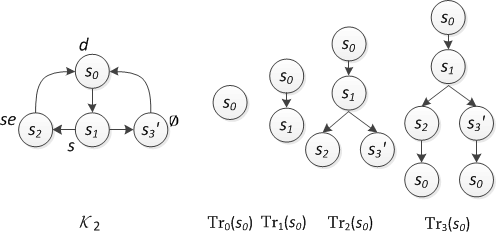
\includegraphics[width=10cm]{chapter05/NK2Tree1.png}
		\caption{初始结构$\mathcal{K}_2$(源于图\ref{Fig:chapter04:v1uv2})及其计算树示意图}\label{fig:K2Tree}
	\end{figure*}
	
	%\begin{figure*}[!htb]
	%	\centering
	%	% Requires \usepackage{graphicx}
	%	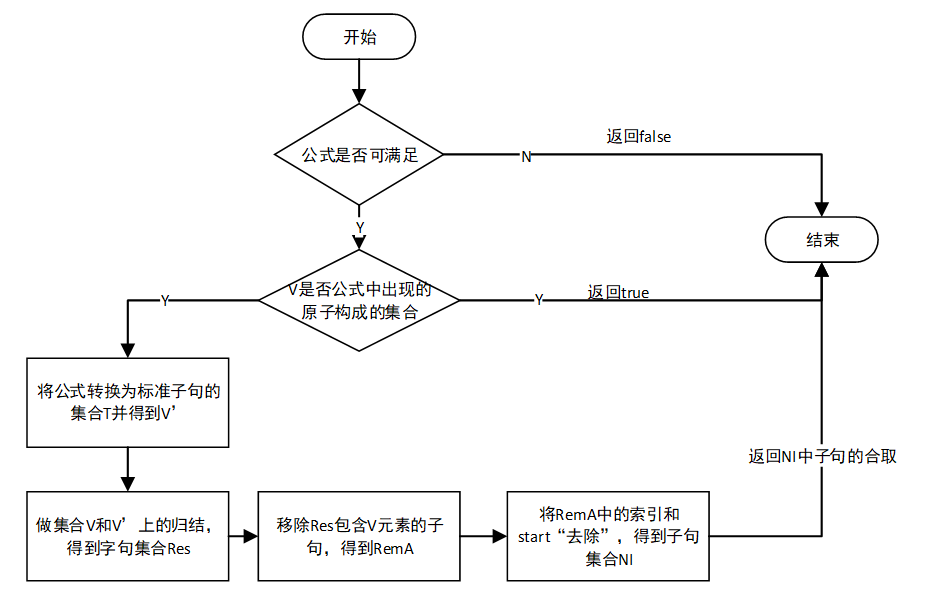
\includegraphics[width=15cm]{chapter04/frame.png}\\
	%	\caption{基于归结的遗忘的主要流程图}
	%	\label{Fig:chapter05:v1uv2}
	%\end{figure*}
	
\end{example}


下面的定理表示,特征公式确实描述了一个初始结构。此时,对系统结构的操作就可转换为对其特征公式的操作,如:下文中的给定系统下的最弱充分条件计算。直观上,特征公式保持了给定初始结构在原子命题集$V$上的所有特性,即:具有$\overline{V}$-互模拟的两个初始结构关于$V$的特征公式逻辑等价。

\begin{theorem}\label{CF}
	令$V\subseteq \Ha$、$\Hm=(S,R,L,s_0)$且$\Hm'=(S',R', L',s_0')$,则:
	\begin{itemize}
		\item[(i)] $(\Hm',s_0') \models {\cal F}_V({\cal M},s_0)
		\text{ 当且仅当 }
		({\cal M},s_0) \lrto_{\overline V} ({\cal M}',s_0')$;
		
		\item[(ii)] 若$s_0 \lrto_{\overline V} s_0'$则${\cal F}_V(\Hm, s_0) \equiv {\cal F}_V(\Hm', s_0')$。
	\end{itemize}
	
\end{theorem}
\begin{proof}
	(i) 令${\cal F}_V(\Hm, s_0)$为$(\Hm, s_0)$关于$V$的特征公式。显然,$\IR({\cal F}_V(\Hm, s_0), \overline V)$。为了证明上述结论成立,首先证明$(\Hm, s_0) \models {\cal F}_V(\Hm, s_0)$。
	
	令$c={ch({\cal M},V)}$,由引理\ref{Bn:to:Tn}可知$(\Hm, s_0) \models {\cal F}_V(\Tr_c(s_0))$。下证特征公式里的另一部分,即:$(\Hm, s_0) \models \bigwedge_{s\in S} \ALL\GLOBAL\ G(\Hm, s)$,其中
	\[G(\Hm, s) = {\cal F}_V(\Tr_c(s)) \rto \left(\bigwedge_{(s,s_1) \in R} \EXIST \NEXT {\cal F}_V(\Tr_c(s_1))\right)\wedge \ALL \NEXT \left(\bigvee_{(s,s_1) \in R} {\cal F}_V(\Tr_c(s_1))\right).\]
	
	为此,下面证明$(\Hm, s_0) \models \ALL\GLOBAL\ G(\Hm, s)$。考虑下面两种情况:
	\begin{itemize}
		\item  若$(\Hm, s_0) \not \models {\cal F}_V(\Tr_c(s))$,显然$(\Hm, s_0) \models G(\Hm, s)$;
		\item 若$(\Hm, s_0) \models {\cal F}_V(\Tr_c(s))$:\\
		$(\Hm, s_0) \models {\cal F}_V(\Tr_c(s))$\\
		$\Rto$  $s_0 \lrto_{\overline V} s$ \hfill (引理\ref{div_s})
		
		$\forall (s, s_1)\in R$:\\
		$(\Hm, s_1) \models {\cal F}_V(\Tr_c(s_1))$  \hfill  ($s_1 \lrto_{\overline V} s_1$)\\
		$\Rto$ $(\Hm, s) \models \bigwedge_{(s,s_1)\in R}\EXIST \NEXT {\cal F}_V(\Tr_c(s_1))$\\
		$\Rto$ $(\Hm, s_0) \models$ $\bigwedge_{(s,s_1)\in R}\EXIST \NEXT {\cal F}_V(\Tr_c(s_1))$    \qquad  ($\IR(\bigwedge_{(s,s_1)\in R}\EXIST \NEXT {\cal F}_V(\Tr_c(s_1)), \overline V)$, $s_0 \lrto_{\overline V} s$)
		
		$\forall (s, s_1) \in R$:\\
		$(\Hm, s_1) \models \bigvee_{(s, s_2)\in R}{\cal F}_V(\Tr_c(s_2))$\\
		$\Rto$ $(\Hm, s) \models \ALL \NEXT \left( \bigvee_{(s, s_2)\in R} {\cal F}_V(\Tr_c(s_2)) \right)$ \\
		$\Rto$ $(\Hm, s_0) \models$  $\ALL \NEXT \left( \bigvee_{(s, s_2)\in R} {\cal F}_V(\Tr_c(s_2)) \right)$     ($\IR(\ALL \NEXT \left( \bigvee_{(s, s_2)\in R} {\cal F}_V(\Tr_c(s_2)) \right), \overline V)$, $s_0 \lrto_{\overline V} s$)\\
		$\Rto$ $(\Hm, s_0) \models G(\Hm, s)$。\\
		% where $s_i$ and $s_j$ are the successors of $s$.
	\end{itemize}
	
	对任意其它能从$s_0$可达的状态$s'$,都可以类似地证明$(\Hm,s')\models G(\Hm, s)$。
	因此,对任意$s\in S$,$(\Hm, s_0) \models \ALL\GLOBAL\ G(\Hm, s)$,从而$(\Hm, s_0) \models {\cal F}_V(\Hm, s_0)$。
	
	下面从两个方面证明(i)成立:
	
	$(\Lto)$ 证明:若$s_0 \lrto_{\overline V} s_0'$,则$(\Hm',s_0') \models {\cal F}_V(\Hm,s_0)$。因为$(\Hm, s_0) \models {\cal F}_V($ $\Hm, s_0)$且 $\IR({\cal F}_V$ $(\Hm, s_0), \overline V)$,由定理\ref{thm:V-bisimulation:EQ}可知
	$(\Hm',s_0') \models {\cal F}_V(\Hm,s_0)$。
	
	$(\Rto)$ 证明:若$(\Hm',s_0') \models {\cal F}_V(\Hm,s_0)$,则$s_0 \lrto_{\overline V} s_0'$。为此,下面证明对任意$n \geq 0$,$Tr_n(s_0) \lrto_{\overline V} Tr_n(s_0')$。
	
	
	\textbf{基始($n=0$):} 由特征公式的定义,显然$Tr_0(s_0) \equiv Tr_0(s_0')$成立。
	
	\textbf{归纳步骤($n>0$):} 假定对任意$k > 0$,都有$\Tr_k(s_0) \lrto_{\overline V} \Tr_k(s_0')$,下面证明$\Tr_{k+1}(s_0)$ $\lrto_{\overline V} \Tr_{k+1}(s_0')$。令$(s_0, s_1), (s_1, s_2)$, $\dots$, $(s_{k-1}, s_k) \in R$且$(s_0', s_1'), (s_1', s_2'), \dots, (s_{k-1}', s_k') \in R'$,即对于任意$0 \leq i \leq k-1$,$s_{i+1}$($s_{i+1}'$)是$s_i$($s_i'$)的直接后继状态。
	由归纳假设可知,只需证明$\Tr_1(s_k) \lrto_{\overline V} \Tr_1(s_k')$。
	
	(a) 由归纳假设可知$L(s_k) - \overline V = L'(s_k') - \overline V$。
	
	在讨论其它点时,首先考虑下面事实(\textbf{fact}):\\
	$(\Hm',s_0') \models {\cal F}_V(\Hm,s_0)$\\
	$\Rto$ $\forall s'\in S'$,$\forall s\in S$,\\ $(\Hm', s')\models {\cal F}_V(\Tr_c(s)) \rto$  $\left(\bigwedge_{(s,s_1)\in R} \EXIST \NEXT {\cal F}_V(\Tr_c(s_1))\right)\wedge \ALL \NEXT \left( \bigvee_{(s,s_1)\in R} {\cal F}_V(\Tr_c(s_1))\right)$  \\
	(I) $(\Hm', s_0') \models {\cal F}_V(\Tr_c(s_0)) \rto \left(\bigwedge_{(s_0, s_1) \in R} \EXIST \NEXT {\cal F}_V(\Tr_c(s_1))\right)$ $\wedge$ $\ALL \NEXT \left(\bigvee_{(s_0, s_1) \in R} {\cal F}_V(\Tr_c(s_1)) \right)$     \\
	(II) $(\Hm', s_0') \models {\cal F}_V(\Tr_c(s_0)))$  \hfill  (已知)\\
	(III) $(\Hm', s_0') \models \left(\bigwedge_{(s_0, s_1) \in R} \EXIST \NEXT {\cal F}_V(\Tr_c(s_1))\right)$ $\wedge$ $\ALL \NEXT \left(\bigvee_{(s_0, s_1) \in R} {\cal F}_V(\Tr_c(s_1)) \right)$  \hfill  ((I),(II))\\
	
	% It is apparent that $L'(s_0') - \overline V = L(s_0) - \overline V$;\\
	(b) 下证$\forall (s_k, s_{k+1}) \in R$,存在$(s_k', s_{k+1}') \in R'$,使得$L(s_{k+1}) - \overline V = L'(s_{k+1}') - \overline V$。\\
	(1) $(\Hm', s_0') \models \bigwedge_{(s_0, s_1) \in R} \EXIST \NEXT {\cal F}_V(\Tr_c(s_1))$  \hfill  (III)\\
	(2) $\forall (s_0, s_1) \in R$,$\exists (s_0', s_1') \in R'$,使得 $(\Hm', s_1') \models {\cal F}_V(\Tr_c(s_1))$  \hfill  (1)\\
	(3) $\Tr_c(s_1) \lrto_{\overline V} \Tr_c(s_1')$  \hfill  ((2), 引理\ref{Bn:to:Tn}) \\
	(4) $L(s_1) - \overline V = L'(s_1') - \overline V$  \hfill   ((3), $c \geq 0)$\\
	(5) $(\Hm', s_1') \models {\cal F}_V(\Tr_c(s_1)) \rto \left(\bigwedge_{(s_1,s_2)\in R} \EXIST \NEXT {\cal F}_V(\Tr_c(s_2))\right) \wedge \ALL \NEXT \left(\bigvee_{(s_1,s_2)\in R} {\cal F}_V(\Tr_c(s_2))\right)$     \hfill  \textbf{(fact)}\\
	(6) $(\Hm', s_1') \models \left(\bigwedge_{(s_1,s_2)\in R} \EXIST \NEXT {\cal F}_V(\Tr_c(s_2))\right) \wedge \ALL \NEXT \left(\bigvee_{(s_1,s_2)\in R} {\cal F}_V(\Tr_c(s_2))\right)$ \hfill ((2), (5))\\
	%(7) $\dots \dots$ \\
	(7) $(\Hm', s_k') \models \left(\bigwedge_{(s_k,s_{k+1})\in R} \EXIST \NEXT {\cal F}_V(\Tr_c(s_{k+1}))\right) \wedge \ALL \NEXT \left(\bigvee_{(s_k,s_{k+1})\in R} {\cal F}_V(\Tr_c(s_{k+1}))\right)$       \hfill (与(6)类似)\\
	(8) $\forall (s_k, s_{k+1}) \in R$,$\exists (s_k', s_{k+1}') \in R'$,使得$(\Hm', s_{k+1}') \models {\cal F}_V(\Tr_c(s_{k+1}))$  \hfill  (7)\\
	(9) $\Tr_c(s_{k+1}) \lrto_{\overline V} \Tr_c(s_{k+1}')$    \hfill ((8), 引理\ref{Bn:to:Tn}) \\
	(10) $L(s_{k+1}) - \overline V = L'(s_{k+1}') - \overline V$  \hfill   ((9), $c \geq 0)$\\
	
	(c) 下证$\forall (s_k', s_{k+1}') \in R'$,存在$(s_k, s_{k+1})\in R$,使得$L(s_{k+1}) - \overline V = L'(s_{k+1}') - \overline V$。\\
	(1) $(\Hm', s_k') \models \ALL \NEXT \left(\bigvee_{(s_k,s_{k+1})\in R} {\cal F}_V(\Tr_c(s_{k+1}))\right)$  \hfill (上面的(7))\\
	(2) $\forall (s_k', s_{k+1}') \in R'$,$\exists (s_k, s_{k+1}) \in R$,使得$(\Hm', s_{k+1}') \models {\cal F}_V(\Tr_c(s_{k+1}'))$  \hfill (1) \\
	(3) $\Tr_c(s_{k+1}) \lrto_{\overline V} \Tr_c(s_{k+1}')$    \hfill ((2), 引理\ref{Bn:to:Tn}) \\
	(4) $L(s_{k+1}) - \overline V = L'(s_{k+1}') - \overline V$  \hfill   ((3), $c \geq 0)$\\
	
	(ii) 由引理\ref{lem:Vb:TrFormula:Equ}和\ref{div_s}易得。
	
\end{proof}

上文描述了初始结构特征公式的计算,下面给出例\ref{exam:SNCandWSC}的详细计算过程。
\begin{example}[例~\ref{exam:SNCandWSC}的延续]
	%\label{exam:SNCandWSC}
	令$\Ha=\{d,se,sp,s\}$和$V=\{d,se\}$,求$s$在$V$和初始结构${\cal K} = (\Hm,s_0)$上的WSC,其中$\Hm$为例~\ref{car_manufacturing}中初始状态为$s_0$的汽车制造企业模型结构。
	
	由定理~\ref{thm:inK:SNC}可知,$s$在$V$和初始结构${\cal K} = (\Hm,s_0)$上的WSC为$\neg \CTLforget({\cal F}_{\Ha}({\cal K}) \wedge \neg s, \{s\} \cup \{sp\})$。
	\begin{align*}
		&	\CTLforget({\cal F}_{\Ha}({\cal K}) \wedge \neg s, \{s\} \cup \{sp\})\\
		&	\equiv \CTLforget(\CTLforget({\cal F}_{\Ha}({\cal K}) \wedge \neg s, \{sp\}), \{s\})\\
		&	\equiv \CTLforget(\CTLforget({\cal F}_{\Ha}({\cal K}), \{sp\})\wedge \neg s, \{s\}).
	\end{align*}
	
	${\cal K}_1 \models \CTLforget({\cal F}_{\Ha}({\cal K}), \{sp\})$\\
	$\LRto$ 存在${\cal K}_1' \lrto_{\{sp\}} {\cal K}_1$,使得${\cal K}_1' \models {\cal F}_{\Ha}({\cal K})$和\\
	$\LRto$ 存在${\cal K}_1' \lrto_{\{sp\}} {\cal K}_1$,使得${\cal K}_1' \lrto_{\emptyset} {\cal K}$\\
	$\LRto$ 存在${\cal K}_1' \lrto_{\{sp\}} {\cal K}$和${\cal K}_1' \models {\cal F}_{V\cup \{s\}}({\cal K})$ \hfill (定理~\ref{CF})\\
	$\LRto$ ${\cal K}_1 \models {\cal F}_{V\cup \{s\}}({\cal K})$。
	
	由此可知,$ \CTLforget({\cal F}_{\Ha}({\cal K}), \{sp\}) \equiv {\cal F}_{V\cup \{s\}}({\cal K})$。所以要计算$\neg \CTLforget({\cal F}_{\Ha}({\cal K}) \wedge \neg s, \{s\} \cup \{sp\})$,只需计算$\neg \CTLforget({\cal F}_{V\cup \{s\}}({\cal K})\wedge \neg s, \{s\})$。令$V' = V \cup \{s\} = \{d,se,s\}$,则$\overline{V'} = \{sp\}$。
	
	
	易知,除了$s_2$和$s_4$是$\overline{V'}$-互模拟的以外,其余都是$V'$-可区分的,且$\dis_{V'}(\Hm, s_i, s_j, 0)$,其中$i\not =j$且$i$和$j$不能同时分别取值2和4。
	因此可以计算$\Hm$关于$V'$的特征数为:
	$$ch(\Hm, V')=\max\{k\mid s,s'\in S \text{ 且 } \dis_{V'}({\cal M},s,s',k)\} = 0\hbox{。}$$
	
	
	所以,可以由以下步骤计算${\cal K}_2$关于$V$的特征公式:
	\begin{align*}
		{\cal F}_{V'}(\Tr_0(s_0)) &= d \wedge \neg se \wedge \neg s, \qquad \qquad \qquad \qquad \quad {\cal F}_{V'}(\Tr_0(s_1)) = \neg d \wedge \neg se \wedge s, \\
		{\cal F}_{V'} (\Tr_0(s_2)) &= {\cal F}_{V'} (\Tr_0(s_4)) = \neg d \wedge se \wedge \neg s,  \qquad  {\cal F}_{V'}(\Tr_0(s_3) = \neg d \wedge \neg se\wedge \neg s,\\
		{\cal F}_{V'}(\Hm, s_0)& \equiv d \wedge \neg se \wedge \neg s \wedge \\
		& \ALL \GLOBAL(d \wedge \neg se \wedge \neg s \rto \ALL\NEXT(\neg d \wedge \neg se \wedge s))\wedge \\
		& \ALL \GLOBAL(\neg d \wedge \neg se \wedge s \rto [\ALL\NEXT((\neg d \wedge se \wedge \neg s) \vee (\neg d \wedge \neg se\wedge \neg s)) \wedge\\ &\EXIST\NEXT(\neg d \wedge se \wedge \neg s) \wedge \EXIST\NEXT (\neg d \wedge \neg se\wedge \neg s)]) \wedge\\
		& \ALL \GLOBAL(\neg d \wedge \neg se\wedge \neg s \rto \ALL\NEXT(d \wedge \neg se \wedge \neg s)) \wedge\\
		& \ALL \GLOBAL(\neg d \wedge se \wedge \neg s \rto \ALL\NEXT(d \wedge \neg se \wedge \neg s)).
	\end{align*}
	令:
	\begin{align*}
		\varphi_1&  = d \wedge \neg se \wedge \neg s \rto \ALL\NEXT(\neg d \wedge \neg se \wedge s)\equiv \neg d \vee se \vee s \vee \ALL\NEXT(\neg d \wedge \neg se \wedge s),\\
		\varphi_2& = \neg d \wedge \neg se \wedge s \rto \ALL\NEXT(\neg d \wedge se \wedge \neg s) \equiv d \vee  se \vee \neg s \vee\\
		& [\ALL\NEXT((\neg d \wedge se \wedge \neg s) \vee (\neg d \wedge \neg se\wedge \neg s)) \wedge\EXIST\NEXT(\neg d \wedge se \wedge \neg s) \wedge \EXIST\NEXT (\neg d \wedge \neg se\wedge \neg s)],\\
		\varphi_3 &=\neg d \wedge \neg se\wedge \neg s \rto \ALL\NEXT(d \wedge \neg se \wedge \neg s)\equiv d \vee se \vee s \vee \ALL\NEXT(d \wedge \neg se \wedge \neg s),\\
		\varphi_4 &= \neg d \wedge se \wedge \neg s \rto \ALL\NEXT(d \wedge \neg se \wedge \neg s)\equiv d \vee \neg se \vee s \vee \ALL\NEXT(d \wedge \neg se \wedge \neg s).
	\end{align*}
	此外,令
	\begin{align*}
		& \psi_1 = \neg d \vee se \vee s && \psi_2 = d \vee  se \vee \neg s \\
		& \psi_3 = d \vee se \vee s && \psi_4 = d \vee \neg se \vee s\\
		& \alpha_1 = \ALL\NEXT(\neg d \wedge \neg se \wedge s) && \alpha_2 = \ALL\NEXT((\neg d \wedge se \wedge \neg s) \vee (\neg d \wedge \neg se\wedge \neg s))\\
		& \alpha_3 = \EXIST\NEXT(\neg d \wedge se \wedge \neg s) \wedge \EXIST\NEXT (\neg d \wedge \neg se\wedge \neg s) && \alpha_4 = \ALL\NEXT(d \wedge \neg se \wedge \neg s)\\
		& \alpha_5 = \ALL\NEXT(d \wedge \neg se \wedge \neg s) && \psi = d \wedge \neg se \wedge \neg s.
	\end{align*}
	则,
	\begin{align*}
		& \psi \wedge \varphi_1 \wedge \varphi_2 \wedge \varphi_3\wedge \varphi_4 
		\equiv (\psi \wedge \psi_1 \wedge \psi_2 \wedge \psi_3 \wedge \psi_4) \vee (\psi \wedge \psi_1 \wedge \psi_2 \wedge \psi_3 \wedge \alpha_5) \vee\\
		& (\psi \wedge \psi_1 \wedge \psi_2 \wedge \alpha_4 \wedge \psi_4) \vee (\psi \wedge \psi_1 \wedge \psi_2 \wedge \alpha_4 \wedge \alpha_5) \vee\\
		& (\psi \wedge \psi_1 \wedge \alpha_2 \wedge \alpha_3 \wedge \psi_3 \wedge \psi_4) \vee (\psi \wedge \psi_1 \wedge \alpha_2 \wedge \alpha_3 \wedge \psi_3 \wedge \alpha_4) \vee \\
		& (\psi \wedge \psi_1 \wedge \alpha_2 \wedge \alpha_3 \wedge \alpha_4 \wedge \psi_4) \vee (\psi \wedge \psi_1 \wedge \alpha_2 \wedge \alpha_3 \wedge \alpha_4 \wedge \alpha_5) \vee\\
		& (\psi \wedge \alpha_1 \wedge \psi_2 \wedge \psi_3 \wedge \psi_4) \vee (\psi \wedge \alpha_1 \wedge \psi_2 \wedge \psi_3 \wedge \alpha_5)\vee\\
		& (\psi \wedge \alpha_1 \wedge \psi_2 \wedge \alpha_4 \wedge \psi_4) \vee (\psi \wedge \alpha_1 \wedge \psi_2 \wedge \alpha_4 \wedge\alpha_5)\vee \\
		& (\psi \wedge \alpha_1 \wedge \alpha_2 \wedge \alpha_3 \wedge \psi_3 \wedge \psi_4) \vee (\psi \wedge \alpha_1 \wedge \alpha_2 \wedge \alpha_3\wedge \psi_3 \wedge \alpha_5) \vee \\
		& (\psi \wedge \alpha_1 \wedge \alpha_2 \wedge \alpha_3 \wedge \alpha_4 \wedge \psi_4) \vee (\psi \wedge \alpha_1 \wedge \alpha_2 \wedge \alpha_3 \wedge \alpha_4 \wedge \alpha_5).\\
		\\
		%\end{align*}
		%\begin{align*}
		& \varphi_1 \wedge \varphi_2 \wedge \varphi_3\wedge \varphi_4 
		\equiv (\psi_1 \wedge \psi_2 \wedge \psi_3 \wedge \psi_4) \vee (\psi_1 \wedge \psi_2 \wedge \psi_3 \wedge \alpha_5) \vee\\
		& (\psi_1 \wedge \psi_2 \wedge \alpha_4 \wedge \psi_4) \vee (\psi_1 \wedge \psi_2 \wedge \alpha_4 \wedge \alpha_5) \vee\\
		& (\psi_1 \wedge \alpha_2 \wedge \alpha_3 \wedge \psi_3 \wedge \psi_4) \vee ( \psi_1 \wedge \alpha_2 \wedge \alpha_3 \wedge \psi_3 \wedge \alpha_4) \vee \\
		& ( \psi_1 \wedge \alpha_2 \wedge \alpha_3 \wedge \alpha_4 \wedge \psi_4) \vee ( \psi_1 \wedge \alpha_2 \wedge \alpha_3 \wedge \alpha_4 \wedge \alpha_5) \vee\\
		& (\alpha_1 \wedge \psi_2 \wedge \psi_3 \wedge \psi_4) \vee ( \alpha_1 \wedge \psi_2 \wedge \psi_3 \wedge \alpha_5)\vee\\
		& (\alpha_1 \wedge \psi_2 \wedge \alpha_4 \wedge \psi_4) \vee ( \alpha_1 \wedge \psi_2 \wedge \alpha_4 \wedge\alpha_5)\vee \\
		& (\alpha_1 \wedge \alpha_2 \wedge \alpha_3 \wedge \psi_3 \wedge \psi_4) \vee (\alpha_1 \wedge \alpha_2 \wedge \alpha_3\wedge \psi_3 \wedge \alpha_5) \vee \\
		& ( \alpha_1 \wedge \alpha_2 \wedge \alpha_3 \wedge \alpha_4 \wedge \psi_4) \vee ( \alpha_1 \wedge \alpha_2 \wedge \alpha_3 \wedge \alpha_4 \wedge \alpha_5).
	\end{align*}
	所以,
	\begin{align*}
		&\neg \CTLforget({\cal F}_{V\cup \{s\}}({\cal K})\wedge \neg s, \{s\}) \\
		& \equiv \neg \CTLforget({\cal F}_{V\cup \{s\}}({\cal K}), \{s\})\\
		& \equiv \neg \CTLforget(\psi \wedge \ALL \GLOBAL(\varphi_1 \wedge \varphi_2 \wedge \varphi_3\wedge \varphi_4),\{s\})\\	
		& \equiv \neg(\CTLforget(\psi \wedge \varphi_1 \wedge \varphi_2 \wedge \varphi_3\wedge \varphi_4, \{s\}) \wedge \ALL \GLOBAL \CTLforget(\varphi_1 \wedge \varphi_2 \wedge \varphi_3\wedge \varphi_4, \{s\}))\\
		& \equiv  \neg \bigg(\Big(d \vee \big((d\vee se) \wedge \ALL\NEXT(d \wedge \neg se)\big) \vee \big((d \vee se \vee \ALL\NEXT \neg d) \wedge \EXIST\NEXT(\neg d \wedge se) \wedge \EXIST\NEXT(\neg d \wedge \neg se)\big) \\
		& \vee (d \wedge \ALL\NEXT(\neg d \wedge \neg se)) \vee \big((d\vee \neg se) \wedge \EXIST\NEXT\neg d\big) \Big) \wedge\\
		& \ALL \GLOBAL\Big(\big((d \vee se) \wedge \ALL\NEXT(d \wedge \neg se)\big) \vee \big(\ALL\NEXT \neg d \wedge \EXIST\NEXT(\neg d \wedge se) \wedge\\
		& \EXIST\NEXT(\neg d \wedge \neg se)\big) \vee \big((d\vee se) \wedge \ALL\NEXT(\neg d \wedge \neg se)\big) \vee \EXIST\NEXT \neg d\Big)
		\bigg)\hbox{。}
	\end{align*}
\end{example}

\subsection{遗忘封闭性及复杂性}\label{chapter06:sec:close}
当$\CTL$公式的长度(符号的个数)为$n$时,由小模型理论可知,定义在状态个数为$k=n8^n$的状态空间${\cal S}=\{s_1,s_2,\dots, s_k\}$上的初始Kripke结构能保证公式的可满足性~\cite{DBLP:journals/jcss/EmersonH85}。
对于其它拥有同样大小的状态空间上的任意初始结构,都能在状态空间${\cal S}$上找到一个初始结构与之互模拟,且由定理\ref{CF}可知它们有相同的特征公式。
因此,只有有限个初始结构作为该公式的候选模型。从而下面结论成立。
%这一事实可以用下面引理表示。

\begin{lemma}\label{lem:models:formula}
	给定$\CTL$公式$\varphi$,下面等式成立:
	\begin{equation*}
		\varphi\equiv \bigvee_{(\Hm, s_0)\in\Mod(\varphi)}{\cal F}_{\cal A}(\Hm, s_0).
	\end{equation*}
\end{lemma}
\begin{proof}
	令$(\Hm', s_0')$为$\varphi$的模型。由定理\ref{CF}可知$(\Hm', s_0') \models {\cal F}_{\Ha}(\Hm', s_0')$,则:
	$$(\Hm', s_0') \models \bigvee_{(\Hm, s_0)\in \Mod(\varphi)} {\cal F}_{\Ha}(\Hm, s_0).$$
	
	另一方面,假定$(\Hm', s_0')$为$\bigvee_{(\Hm, s_0)\in \Mod(\varphi)} {\cal F}_{\Ha}(\Hm, s_0)$的模型。则存在$(\Hm, s_0)\in \Mod(\varphi)$ ,使得 $(\Hm', s_0') \models {\cal F}_{\Ha}(\Hm,$ $s_0)$。由定理\ref{CF}可知$(\Hm, s_0) \lrto_{\emptyset} (\Hm', s_0')$,从而由定理\ref{thm:V-bisimulation:EQ}可知$(\Hm, s_0)$是 $\varphi$的一个模型。
\end{proof}

该结论表明:任意$\CTL$公式都与其模型的特征公式的析取逻辑等价。这对遗忘理论的封闭性提供了重要的理论支撑,即:从公式里遗忘原子命题集$V$中的元素只需找到与给定公式的模型$V$-互模拟的那些模型就能确定遗忘的结果。形式化地,对于给定的公式$\varphi$和原子命题集$V$,从$\varphi$中遗忘$V$中的元素得到的结果为:
\begin{equation*}
	\bigvee_{{\cal K}\in  \{{\cal K}'\mid \exists {\cal K}''\in\Mod(\phi),\ {\cal K}''\lrto_V{\cal K}'\}} {\cal F}_{\overline V}({\cal K}).
\end{equation*}



下面分析遗忘在$\CTL$段$\CTL_{\ALL\FUTURE}$下推理问题的复杂性结果,其中$\CTL_{\ALL\FUTURE}$表示$\CTL$公式只包含时序算子$\ALL \FUTURE$的子类。
这一类公式在并发系统中的互斥和等待等属性描述中有重要作用~\cite{Baier:PMC:2008}。尽管这类公式是相对简单的,但是下面将要说明判定一个模型是否为此类公式遗忘结果的模型是$\textsc{NP}$-完全的。
\begin{proposition}[模型检测]
	\label{modelChecking}
	给定一个结构 $(\Hm,s_0)$、原子命题集$V\subseteq{\cal A}$和公式 $\varphi \in \CTL_{\ALL\FUTURE}$,判定 $(\Hm,s_0)$ 是否为$\CTLforget(\varphi, V)$的模型是 \textsc{NP}-完全的。
\end{proposition}
\begin{proof}
	在$\textsc{NP}$中. 假定$(\Hm,s_0) \models \CTLforget(\varphi,V)$,则存在一个初始结构$(\Hm', s_0')$,使得\ (a) $(\Hm',s_0') \models \varphi$且\ (b) $(\Hm,s_0) \lrto_V (\Hm',s_0')$。已有结果表明:(a)能在$\Hm'$和 $\varphi$的大小的多项式时间内完成~\cite{DBLP:books/daglib/0007403};条件(b)也可用Baier等人的推论 7.45~\cite{Baier:PMC:2008}的方法证明能在多项式时间内完成。
	又因为猜$(\Hm,s_0)$多项式大小的初始结构$(\Hm',s_0')$能在多项式时间内完成。因此,这一问题在$\textsc{NP}$中。
	
	$\textsc{NP}$-难. 已经证明命题逻辑下遗忘的模型检测是$\textsc{NP}$-难的,由于命题逻辑下的遗忘是$\CTL$的一种~\cite{Zhang2008Properties}。因此,上述问题是$\textsc{NP}$-难的。
\end{proof}

关于遗忘的逻辑蕴涵问题也是值得考虑的。下面讨论$\CTL_{\ALL\FUTURE}$段下关于遗忘的逻辑蕴涵问题的复杂性。
下文用记号$\alpha \models^? \beta$表示“$\alpha$是否逻辑蕴涵$\beta$”。

\begin{theorem}[Entailment]
	\label{thm:comF}
	令 $\varphi$和 $\psi$为$\CTL_{\ALL \FUTURE}$中的两个公式, $V$为原子命题集。则:
	\begin{itemize}
		\item[(i)] 判定  $\CTLforget(\varphi, V ) \models^? \psi$是 co-$\textsc{NP}$-完全的,
		\item[(ii)] 判定  $\psi \models^? \CTLforget(\varphi, V)$是 $\Pi_2^{\textsc{P}}$-完全的,
		\item[(iii)] 判定 $\CTLforget(\varphi, V) \models^? \CTLforget(\psi, V)$是 $\Pi_2^{\textsc{P}}$-完全的。
	\end{itemize}
\end{theorem}
\begin{proof}
	(i) co-$\textsc{NP}$-难. 已有结论表明,判定公式$\varphi$是否是可满足的是$\textsc{NP}$-完全的~\cite{meier2009complexity}。令$\psi \equiv \bot$,只需证明$\varphi$是不可满足的,该问题是co-$\textsc{NP}$-难的。所以,原问题是co-$\textsc{NP}$-难的。
	
	在co-$\textsc{NP}$中. 定理\ref{thm:exist}表明$\CTLforget(\varphi, V) \models \psi$当且仅当 $\varphi \models \psi$且 $\IR(\psi, V)$。
	在$\CTL_{\ALL \FUTURE}$中,判定 $\varphi \models \psi$是co-$\textsc{NP}$的~\cite{meier2009complexity}。
	这里证明 $\IR(\psi, V)$是否成立是 co-$\textsc{NP}$的。不失一般性地,假定$\psi$是可满足的,则 $\psi$有一个大小为$|\psi|$的多项式的模型。
	这里讨论该问题的补问题:判定 $\psi$是$V$-有关的,即 $\neg \IR(\psi, V)$。显然,$\neg \IR(\psi, V)$当且仅当存在$\psi$的一个模型 $(\Hm,s_0)$和大小为$|\psi|$的多项式的初始结构 $(\Hm',s_0')$,使得 $(\Hm,s_0) \lrto_V (\Hm',s_0')$且 $(\Hm',s_0') \not \models \psi$。因此,判定$\neg \IR(\psi, V)$是否成立有如下两个步骤:(1)猜两个大小为$|\psi|$的多项式的初始结构$(\Hm,s_0)$和 $(\Hm',s_0')$,使得 $(\Hm,s_0) \models \psi$且 $(\Hm',s_0') \not \models \psi$,和(2)检查 $(\Hm,s_0) \lrto_V (\Hm',s_0')$。
	显然, (1)和(2)都是能在多项式时间内完成的。
	
	(ii) 在$\Pi_2^{\textsc{P}}$中. 考虑这一问题的补问题。猜一个大小为$|\psi|$的多项式的$\psi$的 模型 $(\Hm,s_0)$且检查 是否 $(\Hm, s_0) \not \models \CTLforget(\varphi, V)$。
	由命题\ref{modelChecking} 可知这一问题在 $\Sigma_2^{\textsc{P}}$中。因此,原问题在$\Pi_2^{\textsc{P}}$中。
	
	$\Pi_2^{\textsc{P}}$-难. 令$\psi \equiv \top$。 则这一问题被规约为判定$\CTLforget(\varphi, V)$的有效性问题。 
	由于命题遗忘是$\CTL$遗忘的特殊情形,因此该问题的困难属性直接来源于文献\cite{DBLP:journals/jair/LangLM03}。
	
	(iii) 在$\Pi_2^{\textsc{P}}$中. 假定 $\CTLforget(\varphi, V) \not \models \CTLforget(\psi, V)$。则存在一个初始结构 $(\Hm,s) 
	\models \CTLforget(\varphi, V)$ 且$(\Hm,s) \not \models \CTLforget(\psi, V)$,即存在一个初始结构$(\Hm_1,s_1) \lrto_V (\Hm,s)$,使得 $(\Hm_1, s_1) \models \varphi$ 但是对其它$(\Hm, s) \lrto_V (\Hm_2,s_2)$,使得 $(\Hm_2, s_2) \not \models \psi$。
	由命题\ref{modelChecking}的证明可知,$(\Hm,s)$和 $(\Hm_1,s_1)$ 能在$|\varphi|$、$|\psi|$和$|V|$的多项式时间内完成。 
	显然,猜使得$(\Hm_1,s_1) \lrto_V (\Hm,s)$ 成立的大小为$|\varphi|$多项式的 $(\Hm,s)$和 $(\Hm_1,s_1)$ 可以在多项式时间内完成,且 对任意 $(\Hm, s) \lrto_V (\Hm_2,s_2)$,检查 $(\Hm_2,s_2) \not \models \psi$可以在 $|\psi|$和 $|\Hm_2|$的多项式时间内完成。
	因此,该问题是 $\Pi_2^{\textsc{P}}$的。
	
	$\Pi_2^{\textsc{P}}$-难. 由于 $\IR(\CTLforget(\psi, V), V)$,因此 $\CTLforget(\varphi, V) \models \CTLforget(\psi, V)$当且仅当 $\varphi \models \CTLforget(\psi,$ $V)$。 所以由(ii)不难证明该问题。
\end{proof}



定理\ref{thm:comF}蕴涵下列结论。
\begin{corollary}
	令 $\varphi$和 $\psi$为 $\CTL_{\ALL \FUTURE}$中的两个公式,$V$原子公式集。则
	\begin{itemize}
		\item[(i)] 判定 $\psi \equiv^?\CTLforget(\varphi, V)$是 $\Pi_2^{\textsc{P}}$-完全的,
		\item[(ii)] 判定 $\CTLforget(\varphi, V) \equiv^? \varphi$是 co-$\textsc{NP}$-完全的,
		\item[(iii)] 判定 $\CTLforget(\varphi, V) \equiv^? \CTLforget(\psi, V)$是$\Pi_2^{\textsc{P}}$-完全的。
	\end{itemize}
\end{corollary}


\subsection{基于模型的遗忘算法}\label{chapter06:sec:algm}
这里基于模型的遗忘算法,该算法与第\ref{cha4:sec:alg}节中基于语法的算法不同。本小节的算法通过计算所有可能的模型来计算遗忘,且其正确性可由引理\ref{lem:models:formula}和定理\ref{CF}保证。


\begin{algorithm}[tb]
	\caption{\small 基于模型的$\CTL$遗忘过程}%A Model-based \CTL\ Forgetting Procedure}
	\label{alg:compute:forgetting:by:VB}
	\LinesNumbered
	\KwIn{$\CTL$公式$\varphi$和原子命题集$V$}%A \CTL formula $\varphi$ and a set $V$ of atoms}
	\KwOut{$\CTLforget(\varphi, V)$}% ????
	$\psi \lto \bot$\;
	\ForEach{$\cal A$ 和$\cal S$上的初始结构$\cal K$}{
	%\ForEach{initial \MPK-structure $\cal K$ (over $\cal A$ and $\cal S$)}{
		\lIf{${\cal K}\not\models\varphi$}{{\bf continue}} \\
		\ForEach{满足${\cal K}\lrto_{ V}{\cal K}'$的初始结构${\cal K}'$}{
			$\psi \lto \psi \lor {\cal F}_{\overline V}({\cal K}')$\;
		}
	}
	\Return $\psi$\;
\end{algorithm}



下面的例子来源于研究背景和意义部分。这里给出如何计算从规范中遗忘一些原子命题。 
\begin{example}\label{ex:6}
	对于图\ref{BVM}中的 ${\cal K}_1$,假定一个已知的规范(性质)为$\alpha = \EXIST\FUTURE(se \wedge sp)$。显然 ${\cal K}_1$满足 $\alpha$。若想移除掉 $sp$,即从 $\alpha$中遗忘 $sp$,则 $\CTLforget(\alpha,\{ sp\}) \equiv \EXIST\FUTURE se$。此时,该汽车制造公司可以用新的规范$\EXIST\FUTURE se$(这保证驾车最终会被生产)引导未来汽车的生产。
\end{example}


如下所述,通过计算所有可能的模型是非常低效的。但是,这为从理论的角度探索遗忘有重要作用。


\begin{proposition}\label{pro:time:alg1}
	令 $\varphi$为$\CTL$公式,$V\subseteq \Ha$为原子命题集,状态空间大小为 $|{\cal S}|=m$, $|\Ha|=n$,$|V|=x$。则使用算法\ref{alg:compute:forgetting:by:VB}计算从$\varphi$中遗忘$V$中原子的空间复杂度为 $O((n-x)m^{2(m+2)}2^{nm}  \log m)$,且时间复杂性至少与空间复杂性相同。
\end{proposition}
\begin{proof}
	假定每个状态或原子命题占据$\log m$的空间且$n\leq m$,则一个状态对$(s,s')$占据$2\times \log m$位(bit)。对任意$B \subseteq {\cal S}$和$s_0\in B$,构造如下初始结构$(\Hm,s_0)$,其中$\Hm = (B,R,L,s_0)$,则$R$中至多有$\frac{|B|^2}{2}$个状态对且$L$中至多$|B|\times n$个$(s,A)$对($A\subseteq \Ha$)。因此,$(\Hm,s_0)$至多占据$(|B|+|B|^2+|B|\times n)\times \log m$位。此外,对于状态集$B$,初始状态有$|B|$种选择,有$|B|^{|B|}$种关系$R$,$(2^n)^{|B|}$种标签函数$L$。
	
	在最坏的情形下(即$|B|=m$),可构成$m \times  (m^m \times  2^{nm} \times  m)$个初始结构。因此,最多有$m^{m+2} \times  2^{nm}$个初始结构,且最多花费$(m^{m+2} \times  2^{nm} \times  (m + m^2 + nm))\times  \log m$位。
	
	令 $k = n-x$,对任意有$i\geq 1$个状态的初始结构${\cal K} = (\Hm,s_0)$,其中$\Hm = (B,R,L,s_0)$。
	在最坏的情形下(即$ch(\Hm,V) = i$时),需要$N(i) = P_i(s_0) + i \times  (P_i(s) + i \times P_i(s'))$位来存储${\cal K}$在$\overline{V}$上的特征公式。
	其中$s',s\in B$,$P_i(y)$是存储${\cal F}_{\overline{V}}(\Tr_i(y))$($y\in B$)所用的空间(这里假定$\EXIST\NEXT$和$\ALL\NEXT$使用了相同的存储单位)。
	
	${\cal F}_{\overline{V}}(\Tr_i(y))$($0\leq n \leq i$)被递归地定义如下:
	\begin{align*}
		&(1) n=0,  \qquad P_0(y) = k\\
		&(2) n=1, \qquad  P_1(y) = k + i\times k = k + i\times P_0(y)\\
		&(3) n=2, \qquad P_2(y) = k + i\times (k + i\times k) = k+i\times P_1(y)\\
		& \dots \qquad \qquad \dots\\
		&(i+1) n = i, \quad P_i(y) = k + i \times  P_{i-1}(y).
	\end{align*}
	
	因此,有
	\begin{align*}
		P_i(y) & = k + i\times k + i^2 \times  k + \dots + i^i \times  k = \frac{i^i -1}{i-1} k,\\
		N(i) & = P_i(s_0) + i\times  (P_i(s) + i \times  P_i(s'))\\
		& = (i^2 + i +1) P_i(y) \\
		& = (i^2 + i+1)\frac{i^i -1}{i-1} k.
	\end{align*}
	
	在最坏的情形下(即具有$m$个状态的初始结构)有$m^{m+2} \times  2^{nm}$个初始结构,需要$(m^{m+2} \times  2^{nm} \times  N(m)) \times  \log m$位来存储遗忘的结果。
	
	因此,空间复杂性为$O((n-x)m^{2(m+2)}2^{nm}\times  \log m)$。
\end{proof}



\section{基于归结的遗忘计算方法}
\label{chapter05:sec:resolution}
	已有结果显示,任意$\CTL$公式可以转换为$\CTLsnf$子句集。归结是一种以子句为计算对象的判断可满足性的方法。本章提出一种基于归结的计算遗忘的方法,
	其主要思想是:首先,将给定的$\CTL$公式转换为$\CTLsnf$子句集(这一部分在第\ref{chapter02}章已经给出了详细的介绍;其次,在相应的原子命题集$V$上使用归结规则得到归结结果;最后,“消除”之前引入的索引和$\start$,最终得到遗忘的结果。其主要流程图如图\ref{Fig:chapter05:v1uv2}所示。
	正如本章所要说明的那样,$\CTL$不具有均匀插值这一属性,基于归结的方法在有的情况下是不能计算出遗忘结果的。然而,在有些$\CTL$子类下,本章提出的方法能够计算出其遗忘结果。
\begin{figure*}[!htb]
	\centering
	% Requires \usepackage{graphicx}
	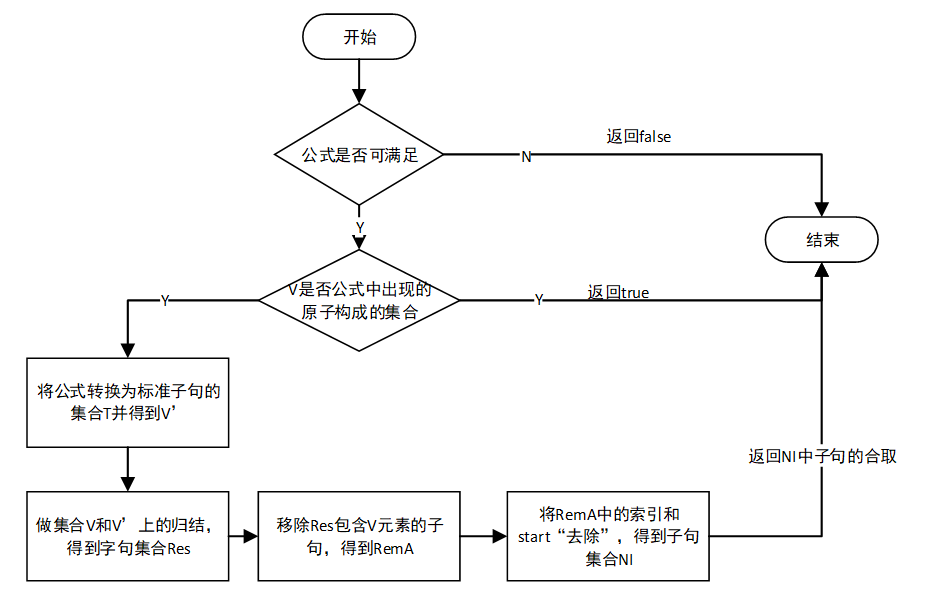
\includegraphics[width=15cm]{chapter04/frame.png}\\
	\caption{基于归结的遗忘的主要流程图}
	\label{Fig:chapter05:v1uv2}
\end{figure*}

%虽然在第\ref{chapter02}章详细介绍了命题逻辑和模态逻辑S5下基于归结的计算遗忘的方法,但值得注意的是$\CTL$公式没有像这两种逻辑一样有标准的自身语言子句形式,而$\CTL$的子句是有索引的。这就注定了$\CTL$下基于归结的遗忘与上述两者的不同,而且也应该要复杂一些(虽有不同,但也可以借鉴)。
本章展示如何使用第\ref{chapter02:CTLres}节中表\ref{tab:res}中的归结规则来计算$\CTL$下的遗忘。
为了计算从$\CTL$公式$\varphi$中遗忘集合$V$中的原子命题,
%为了实现这一目标,
需要解决如下两个主要问题:
\begin{itemize}
	\item[(1)] 如何表示$\CTL$公式和带索引的$\CTL$公式之间的关系?如在第\ref{chapter02}章中所说,将一个$\CTL$公式转换为$\CTLsnf$子句集会引入新的原子命题和索引。虽然已有的研究说明,$\CTL$公式可以转换为带索引的公式集并保证其可满足性,然而并没有表明这两种形式的公式之间的模型具有怎样的联系。
	本章从互模拟等价的角度探讨$\CTL$公式和归结等过程得到的(带索引)公式之间的联系,为计算遗忘提供理论基础。
	%本章给出一种扩展的互模拟定义,以描述两种公式的模型之间的关系。
	\item[(2)] 如何“移除”无关的原子命题(包括需要遗忘的原子命题和转换过程中引入的新的原子命题),以及如何“消除”索引?为此,本章给出“移除”原子命题的一般操作,并提出一种一般化的Ackermann引理。为了“消除”索引,探索几个逻辑等价关系。%,详见第\ref{cha4:sec:resf}节。
	%对应算法\ref{alg:compute:forgetting:by:Resolution}中的$\emph{Removing\_index}(\emph{RemA})$过程。
\end{itemize}

%此外,详细描述基于Prolog上述算法的实现并分析实验结果。

本章其余部分组织如下:首先,在第\ref{cha5:subsec:resf}节详细介绍$\CTL$-forget各个过程及算法复杂性;其次,在第\label{cha5:subsec:prolog}节介绍基于Prolog的$\CTL$-算法的实现;最后,在第\ref{cha5:subsec:expriment}节给出并分析实验结果。
\subsection{基于归结的算法$\CTL$-forget}
\label{cha5:subsec:resf}
通过上述分析,本节主要描述如何使用基础知识部分说的$R_{\CTL}^{\succ,S}$归结系统对要遗忘的原子命题做归结,然后如何将归结后得到的结果等价转换为$\CTL$公式。
\subsubsection{$\CTL$归结$\Unfolding$}

这部分给出如何使用归结规则(表\ref{tab:res})来计算$\CTL$中的遗忘。
这个过程的主要思想是:将转换过程中获得的$\CTLsnf$子句在表\ref{tab:res}中归结规则上做穷尽的归结,即直到不产生新的归结结果。值得注意的是,该归结过程涉及的归结原子命题包括:需要遗忘的原子命题和转换过程中引入的新的原子命题。

令$T$为$\CTLsnf$子句集,$p$为原子命题。$T$在$p$上的\emph{展开}(记为$\Unfolding(T,p)$)是集合$T$和如下集合的并集:
\[\{\alpha\mid \mbox{$\alpha$ 是 $T$ 中的公式关于文字 $l\in\{p,\neg p\}$ 的归结结果}\}.  \]
对于原子命题集$V$,定义$\Unfolding(T,\emptyset)=T$且$\Unfolding(T,\{p\}\cup V)=\Unfolding(\Unfolding(T,p), V)$。
直观上,$T$在$p$上的展开是对$p$做穷尽的归结,即:直到对$p$使用规则{\bf SRES1-8}不再产生新的$\CTLsnf$子句为止(即使使用了重写规则和可能规则之后也不会产生新的子句)。


下面的命题展示了对任意$\CTL$公式$\varphi$,从 $\Unfolding(T_\varphi,V)$ 中移除掉含有$V$中元素的子句得到的结果在不考虑$V$中元素和新引入的元素的情况下是互模拟等价的。
下文中记$\emph{ERes}(\varphi,V) = \{\alpha\in \Unfolding(T_\varphi,V)\mid \Var(\alpha)\cap V=\emptyset\}$。
\begin{proposition}\label{pro:resEQ}
	令 $\varphi$ 为一个 $\CTL$公式,$V\subseteq\cal A$为原子命题集。则
	$T_\varphi \equiv_U\emph{ERes}(\varphi,V)$,其中  $U=\Var(\Unfolding(T_\varphi,V))-(\Var(\varphi)-  V)$。
\end{proposition}
\begin{proof}
	从两个方面来证明这一结论:\textbf{(F1)} $T_\varphi \equiv_U \Unfolding(T_\varphi,V)$, \textbf{(F2)} $\Unfolding(T_\varphi,V) \equiv_{U} \emph{ERes}(\varphi,V)$。
	为此,定义如下 由$\CTLsnf$ 子句集构成的序列: $T_0=T_{\varphi}, T_1, T_2, \dots, T_n = \Unfolding(T_\varphi,V)$,其中
	$T_{i+1} = T_i \cup R_i$ ($0\leq i < n$)、 $R_i$ 是对$\Pi \subseteq T_i$使用一条匹配的规则$r$且该规则归结的原子命题为$p\in V$,这一过程记为 $\Pi \rto_r R_i$。
	\\
	
	\textbf{(F1)} 为了证明$T_\varphi \equiv_U \Unfolding(T_\varphi,V)$,只需证明对任意 $0\leq i < n$,有$T_i \equiv_{U} T_{i+1}$。
	
	
	
	(1) 若 $r\in \{\textbf{(SRES1)},$ $\dots,$ $\textbf{(SRES8)},$ $(\textbf{RW1}),$ $(\textbf{RW2})\}$,则$T_i \equiv_{\{p\}} T_{i+1}$,其中。
	
	
	一方面,显然 $\Pi \models R_i$,所以 $T_i \models T_{i+1}$。另一方面 $T_i\subseteq T_{i+1}$,所以 $T_{i+1} \models T_i$。
	
	(2) 下证若$\Pi \rto_r R_i$且 $r=$\textbf{(ERES1)},
	则 $T_i \equiv_{\{l, w_{\neg l}^{\ALL}\}} T_{i+1}$,其中 $l = p$或 $l = \neg p$,$w_{\neg l}^{\ALL}$是与子句$Q \rto \ALL \FUTURE \neg l$相关的新的原子命题,$l$是文字(即:$p$或者$\neg p$)。
	
	已有结果表明$\Pi \models R_i$~\cite{bolotov2000clausal},因此,$T_{i+1}=T_i \cup \Lambda_{\neg l}^{\ALL}$,其中$\Lambda_{\neg l}^{\ALL}$是通过使用表\ref{tab:trans}中的转换规则作用到$R_i$上得到的$\CTLsnf$子句集~\cite{zhang2009refined}。显然,对所有$(\Hm_1,s_1) \in \Mod(T_i= X \cup \Pi)$都存在一个$(\Hm_2, s_2)\in \Mod(T_{i+1}=T_i \cup \Lambda_{\neg l}^{\ALL})$,使得$(\Hm_1, s_1) \lrto_{\tuple{\{p, w_{\neg l}^{\ALL}\}, {\O}}} (\Hm_2, s_2)$,且对任意$(\Hm_2, s_2)\in \Mod(T_{i+1}=T_i \cup \Lambda_{\neg l}^{\ALL})$,存在一个$(\Hm_1,s_1) \in \Mod(T_i= X \cup \Pi)$,使得$(\Hm_1, s_1) \lrto_{\{p, w_{\neg l}^{\ALL}\}} (\Hm_2, s_2)$。
	又$\{p, w_{\neg l}^{\ALL}\} \subseteq U$,由命题\ref{prop:transform:V:EQ}可知$T_i \equiv_{U} T_{i+1}$。
	
	当规则为$\textbf{(ERES2)}$时可以类似地证明。
	
	总之,$V\subseteq U$.因此,由推论\ref{cor:eqbi}(iii)可知,对任意 $0 \leq i < n$,有$T_i \equiv_U T_{i+1}$。
	又因为$\equiv_U$为等价关系,所以$T_{\varphi} \equiv_U \Unfolding(T_\varphi,V)$。
	
	
	
	\textbf{(F2)} 假设 $V=\{p\}$, $C_i$ ($i=1,2$)为经典子句,  $l = p$ 或 $l = \neg p$。
	显然 $\Unfolding(T_\varphi,V) \models \emph{ERes}(\varphi,V)$,这里证明对任意 ${\cal K}=(\Hm, s)\in \Mod(\emph{ERes}(\varphi,V))$ (其中$\Hm=(S, R, L, [\_], s)$),存在一个初始$\Ind$-结构 ${\cal K}'=(\Hm', s')$,使得 ${\cal K} \lrto_{U} {\cal K}'$ 且 ${\cal K}' \models \Unfolding(T_\varphi,V)$。
	
	
	因为$p$只出现在 $\CTLsnf$子句的右手边,从以下几点证明上述结论成立。
	
	(1) 假定 $\Unfolding(T_\varphi,V)$有全局子句,则对于任意 $C=\top\rto C_1 \vee l \in \Unfolding(T_\varphi,V)$:
	
	(a) 如果不存在 $C'\in \Unfolding(T_\varphi,V)$,使得 $C$ 和 $C'$ 在 $p$上是可归结的,则 $\Unfolding(T_\varphi,V)$中不存在除了 $Pt$-某时 子句之外的子句 $C'$ 包含文字 $\neg l$,其中 $Pt\in \{\ALL, \EXIST\}$。
	
	若对任意其它的子句$C'$, $p\not \in \Var(C')$,则对任意 ${\cal K}=(\Hm, s)\in \Mod(\emph{ERes}(\varphi,V))$,如下构造 $(\Hm',s')$:令 $\Hm'= (S, R, L',[\_], s)$ (即 $s'=s$),其中$L'$ 与 $L$ 一样,除了对任意 $s_1\in S$,若 $(\Hm, s_1) \not \models C_1 \vee l$则“若 $l=p$令 $L'(s_1) = L(s_1) \cup \{p\}$,否则令 $L'(s_1) = L(s_1) - \{p\}$”。
	显然 $(\Hm, s) \lrto_{\{p\}} (\Hm', s')$ 和 $(\Hm', s') \models C' \wedge C$。
	
	若 $C'= Q\rto Pt \FUTURE \neg l$,不失一般性地,令 $l=p$。对任意 ${\cal K}=(\Hm, s)\in \Mod(\emph{ERes}(\varphi,$ $V))$,如下构造 $(\Hm',s')$:令$\Hm'=(S, R, L',[\_], s)$,其中 $L'$与 $L$ 相同,除了
	$L'(s) = L(s) \cup \{p\}$,且对任意具有$(s, s')\in R$关系的状态 $s'\in S'$,令 $L'(s) = L(s) - \{p, q\}$,其中 $q \in (\Var(\Unfolding(T_\varphi,$ $V))-\Var(\varphi))$ 是负出现在 $C_1$ 中的原子命题,且对任意其它的非初始状态 $s'' \in S$,$L'(s'') = (L(s'') - \{Q\}) \cup \{p\}$ ($Q$在 $Pt$-某时子句中是一个原子)。显然,$(\Hm, s) \lrto_{\{p,q\}} (\Hm', s')$ 和 $(\Hm', s') \models C' \wedge C$。
	%	 that for each non-initial state $s\in S'$, we have $L'(s) = (L(s) - \{Q\}) \cup \{p\}$ ($Q$ is an atom for $Pt$-sometime clause)
	%
	%if $Q$ is an atom (if $Q$ is a term, then we can delete the atoms which occurring in $Q$ positively and add the atoms which occurring in $Q$ negatively) 
	%	and $L'(s) = L(s) \cup \{p\}$ if $(\Hm, s) \not \models C_1$ else $L'(s) = L(s)$. 
	%	It is easy to check that ${\cal K} \lrto_{V''} {\cal K}'$ and ${\cal K}' \models \Unfolding(T_\varphi,V)$. 
	%	and if $(\Hm,s)  \models \neg Q \wedge C_1$, then let $L'(s) = L(s)$, else ``if $(\Hm,s) \models \neg Q \wedge \neg C_1$, then let $L'(s) = L(s) \cup \{p\}$, else if $(\Hm,s) \models Q \wedge \neg C_1$, then `if $q$ occurs in $C_1$ positively, then let $L'(s) = L(s) - \{p\} - \{q\}$, else let $L'(s) = (L(s) - \{p\}) \cup \{q\}$' ", where $q \in (\Var(C_1) \cap U)$.
	%		It is obvious that $(\Hm, s) \lrto_{\{p,q\}} (\Hm', s')$ and $(\Hm', s') \models C' \wedge C$.
	
	(b) 若存在子句$C'\in \Unfolding(T_\varphi,V)$,使得 $C$和 $C'$在 $p$上是可归结的:
	\begin{itemize}
		\item[(i)] 若 $C'= Q\rto Pt \NEXT (C_2 \vee \neg l)$ (令 $Pt=\ALL$,$Pt = \EXIST$可类似地证明),则有$Q\rto \ALL \NEXT(C_1 \vee C_2) \in \Unfolding(T_\varphi,V)$。因此,对任意 ${\cal K}=(\Hm, s)\in \Mod(\emph{ERes}(\varphi,V))$,如下构造${\cal K}'$ $=(\Hm',s')$: 令 $\Hm'= (S, R, L',[\_]$ $,s)$ (即 $s'=s$),其中 $L'$ 与 $L$一样,除了对任意 $s_1\in S$,若 $(\Hm, s_1) \not \models Q$,则对任意 $(s_1, s_2) \in R$,若 $(\Hm, s_2) \not \models C_1$ 则“若 $l=p$,则令 $L'(s_2) = L(s_2) \cup \{p\}$,否则令 $L'(s_2) = L(s_2) - \{p\}$”,否则,若$(\Hm, s_2) \models  C_1 \wedge \neg C_2$,则“若$l=p$,则令 $L'(s_2) = L(s_2) - \{p\}$,否则令$L'(s_2) = L(s_2) \cup \{p\}$”;否则,若 $(\Hm, s_2) \models \neg C_1 \wedge C_2$,则“若 $l=p$,则令$L'(s_2) = L(s_2) \cup \{p\}$,否则 $L'(s_2) = L(s_2) - \{p\}$”。显然, ${\cal K} \lrto_{\{p\}} {\cal K}'$ 且 ${\cal K}' \models C' \wedge C$。
		\item[(ii)] 若 $C' =  Q\rto Pt \FUTURE \neg l$。不失一般性地,假设 $l=p$。$C$和$C'$在$p$上是可归结的,则一定存在子句集$\{P_1^1 \rto * C_1^1$, \dots, $P_{m_1}^1 \rto * C_{m_1}^1$, $P_1^n \rto * C_1^n$, \dots, $P_{m_n}^1 \rto * C_{m_n}^1 \}$,使得  $*$要么要么为空字符串,要么为$\{\ALL \NEXT, \EXIST_{\tuple{ind}} \NEXT\}$中的一个($\neg C_1 \rto l$为子句集中的一个),使得 $\bigvee_{i=1}^n \bigwedge_{j=1}^{m_i} P_j^i \rto \EXIST \NEXT \EXIST \GLOBAL l$。
		%, hence $\bigvee_{i=1}^n \bigwedge_{j=1}^{m_i} P_j^i \rto l \wedge \EXIST \NEXT \EXIST \GLOBAL l$.
		%This is a contradiction since $C' =  Q\rto Pt \FUTURE \neg l$.
		因此,通过使用规则ERES1 ( ERES2规则类似)可以得到一个子句 $C''=\top \rto \neg Q \vee \neg p \vee C_1$。所以,在使用规则 SRES8在$C$和 $C''$上后得到子句$\top \rto \neg Q \vee C_1$。在这种情况下,对任意 ${\cal K}=(\Hm, s)\in \Mod(\emph{ERes}(\varphi,V))$,如下构造 ${\cal K}'=(\Hm',s')$:令 $\Hm'= (S, R, L', [\_],s)$ (即 $s'=s$),其中 $L'$与$L$一样,除了对任意 $s_1\in S$,若 $(\Hm, s_1) \models Q$,则令 $L'(s_1) = L(s_1) - \{p\}$,否则令 $L'(s_1) = L(s_1) \cup \{p\}$。可以检查 ${\cal K} \lrto_{\{p\}} {\cal K}'$和 ${\cal K}' \models C' \wedge C$。
		\item[(ii)] 可以类似地证明其它类型的子句,且得到${\cal K} \lrto_{U} {\cal K}'$ 和 ${\cal K}' \models \Unfolding(T_\varphi,V)$。
	\end{itemize}
	
	(2) 考虑$Pt$-步 子句的情形。令 $C\in \Unfolding(T_\varphi,V)$为 $Q \rto \ALL \NEXT(C_1 \vee  l)$。不失一般性地,假设存在某些子句$C'\in \Unfolding(T_\varphi,V)$,使得$C$和 $C'$在$p$上是可归结的($l=p$)。
	
	若 $C'= Q_1\rto Pt \NEXT (C_2 \vee \neg l)$ (令$Pt=\EXIST_{ind}$,$Pt = \ALL$的情形可以类似地证明),因此,$Q \wedge Q_1 \rto \EXIST_{ind} \NEXT(C_1 \vee C_2) \in \Unfolding(T_\varphi,V)$。所以,对任意 ${\cal K}=(\Hm, s)\in \Mod(\emph{ERes}(\varphi,V))$,如下构造 ${\cal K}'=(\Hm',s')$:令$\Hm'= (S, R, L', [\_], s)$(即 $s'=s$),其中 $L'$与 $L$一样,除了对任意 $s_1\in S$
	\begin{itemize}
		\item[(i)] 若$(\Hm, s_1) \not \models Q \wedge Q_1$ 则 “若 $(\Hm, s_1) \models \neg Q \wedge Q_1$则(若 对 $(s_1, s_2') \in \pi_s^{\tuple{ind}}$有$(\Hm, s_2') \not \models C_2$  则令 $L'(s_2') = L(s_2') - \{p\}$否则令 $L'(s_2') = L(s_2')$),否则若 $(\Hm, s_1) \models Q \wedge \neg Q_1$则对任意 $(s_1, s_2) \in R$,(若$(\Hm, s_2) \not \models C_1$则令 $L'(s_2) = L(s_2) \cup \{p\}$,否则令 $L'(s_2') = L(s_2')$),否则令 $L'(s_2') = L(s_2')$”。
		\item[(ii)] 否则若 $(\Hm, s_1) \models Q \wedge Q_1$,则对$(s_1, s_2') \in \pi_s^{\tuple{ind}}$有 $(\Hm,s_2') \models C_1 \vee C_2$。因此,若 $(\Hm, s_2')$ $\models C_1 \wedge \neg C_2$则 $L'(s_2') = L(s_2') - \{p\}$,否则若 $(\Hm, s_2') \models \neg C_1 \wedge C_2$则令$L'(s_2') = L(s_2') \cup \{p\}$,否则令 $L'(s_2') = L(s_2')$。对其它满足$(s_1, s_2) \in R$和 $s_2 \not = s_2'$的状态$s_2$,若 $(\Hm, s_1) \models Q$和 $(\Hm, s_2) \models \neg C_1$,则令 $L'(s_2) = L(s_2) \cup \{p\}$,否则令 $L'(s_2') = L(s_2')$。
	\end{itemize}
	显然,${\cal K} \lrto_{\{p\}} {\cal K}'$和 ${\cal K}' \models C' \wedge C$,其中${\cal K}' = (\Hm',s')$。
	
	若 $C' =  Q_1\rto Pt \FUTURE \neg l$(令$Pt=\ALL$,$Pt = \EXIST$的情形可类似地证明)。若 $C$和 $C'$在$p$上是可归结的,则必须存在 一个包含子句$\neg C_1 \rto l$的$\CTLsnf$子句集 $\{P_1^1 \rto * C_1^1$, \dots, $P_{m_1}^1 \rto * C_{m_1}^1$, $P_1^n \rto * C_1^n$, \dots, $P_{m_n}^1 \rto * C_{m_n}^1 \}$,使得 $*$为空字符串或集合 $\{\ALL \NEXT, \EXIST_{\tuple{ind}} \NEXT\}$中的一个,且 $\bigvee_{i=1}^n \bigwedge_{j=1}^{m_i} P_j^i \rto \EXIST \NEXT \EXIST \GLOBAL l$。
	%	Therefore, we get clause $C''=\top \rto \neg Q \vee \neg p \vee C_1$ by using \textbf{ERES1} (similar for \textbf{ERES2}) and then $\top \rto \neg Q \vee C_1$ by using \textbf{SRES8} on $C$ and $C''$. 
	在这种情况下,对任意${\cal K}=(\Hm, s)\in \Mod(\emph{ERes}(\varphi,V))$,如下构造$(\Hm',s')$:令$\Hm'= (S, R, L', [\_],s)$ (即 $s'=s$),其中  $L'$和 $L$一样,除了对任意状态 $s'\in S'$,若 $L'(s') \models Q$和 $(s',s'') \in R$,则令 $L'(s'') = L(s'') \cup \{p\}$, 若 $(\Hm,s)\models Q_1$,则令 $L'(s) = L(s) - \{p\}$。
	显然,$(\Hm, s) \lrto_{\{p\}} (\Hm', s')$和 $(\Hm',s') \models C' \wedge C$。	
	
	因此,对任意${\cal K}=(\Hm, s)\in \Mod(\emph{ERes}(\varphi,V))$($\Hm=(S, R, L, [\_], s)$),存在一个初始$\Ind$-结构 ${\cal K}'=(\Hm', s')$,使得 ${\cal K} \lrto_{U} {\cal K}'$和 ${\cal K}' \models \Unfolding(T_\varphi,V)$。
	%	 is the same as $L$ except for the initial state $s$ if $(\Hm, s) \models Q_1$ then let $L'(s) = L(s) - \{p\}$ and $L'(s'') = L(s'') \cup \{p\}$ for any non-initial state $s' \in S$ with $L'(s') \models Q$ and $(s',s'') \in R$, else $L'(s'') = L(s'') \cup \{p\}$ for any $s' \in S$ with $L'(s') \models Q$ and $(s',s'') \in R$. It is easy to check that ${\cal K} \lrto_{V''} {\cal K}'$ and ${\cal K}' \models C' \wedge C$.
\end{proof}


\begin{example}[例\ref{examp:Tran}的延续]\label{examp:Res}
	令 $V=\{p,r\}$,则  $\Unfolding(T_\varphi, V\cup \{x,y,z\})$ 除了例\ref{examp:Tran}中的子句,还包含如下子句:
	%	The resolvents, obtained by executing the resolution process on $T_{\varphi}$ of Example\ref{examp:Tran} and $V\cup V'$, are the following clauses (in addition to the ones in Example\ref{examp:Tran}):
	% The \textcolor{red}{resolvent} \textcolor{blue}{resolvents} of $T_{\varphi}$ obtained from Example\ref{examp:Tran} by executing the resolution process on $T_{\varphi}$ and $V\cup V'$ are the following clauses (in addition to the ones in Example\ref{examp:Tran}):
	\begin{align*}
		&(1)\ \start \rto r && (1,2,\textbf{SRES5})
		&&(2)\ \start \rto x \vee y && (1,4,\textbf{SRES5})\\
		% \end{align*}
		% \begin{align*}
		&(3)\ \top \rto \neg z \vee y \vee f \vee m && (3, 4, \textbf{SRES8})
		&&(4)\ y \rto \ALL\NEXT(f\vee m\vee y) && (3,8, \textbf{SRES6})\\
		&(5)\ \top \rto \neg z \vee x \vee p && (4,5, \textbf{SRES8})
		&&(6)\ \top \rto \neg z \vee x \vee q && (4,6, \textbf{SRES8})\\
		&(7)\ y \rto \ALL\NEXT(x\vee p) && (5, 8, \textbf{SRES6})
		&&(8)\ y \rto \ALL\NEXT(x\vee q) && (6, 8, \textbf{SRES6})\\
		&(9)\ \start \rto f\vee m \vee y && (3,(2), \textbf{SRES5})
		% \end{align*}
		% \begin{align*}
		&&(10)\ \start \rto x \vee p && (5,(2),\textbf{SRES5}) \\
		&(11)\ \start \rto x \vee q && (6,(2), \textbf{SRES5})
		&& (12)\ \top \rto p \vee \neg z \vee f \vee m && (5,(3), \textbf{SRES8})\\
		& (13)\ \top \rto q \vee \neg z \vee f \vee m && (6,(3), \textbf{SRES8})
		&&(14)\ y \rto \ALL\NEXT(p \vee f\vee m) && (5, (4), \textbf{SRES6})\\
		&(15)\ y \rto \ALL\NEXT(q \vee f\vee m) && (6, (4), \textbf{SRES6})
		%\end{align*}
		%\begin{align*}
		&&(16)\ \start \rto f\vee m \vee p && (5, (9), \textbf{SRES5}) \\
		&(17)\ \start \rto f\vee m \vee q && (6, (9), \textbf{SRES5})
	\end{align*}
	
	在从 $\Unfolding(T_\varphi, V\cup \{x,y,z\})$中移除掉包含 $V$中元素的子句后,得到 $\emph{ERes}(\varphi,V)$,其包含如下子句:
	\begin{align*}%{llll}
		&\start\rto z, \quad \start \rto f\vee m \vee q, \quad  \start \rto x \vee y, \quad \start \rto q \vee x, \quad	\start \rto f\vee m \vee y, \\
		& \top \rto f \vee m \vee \neg x, \quad		\top \rto q \vee f \vee m\vee \neg z,
		\quad  	\top \rto f \vee m \vee \neg z \vee y,\\
		& \top \rto q \vee x\vee \neg z, \quad 	\top \rto x \vee y \vee \neg z, \quad 	\top \rto q\vee\neg y , \quad z \rto \ALL \FUTURE x, \\
		& y \rto \ALL\NEXT(q \vee f\vee m), \quad  y \rto \ALL\NEXT(x\vee q), \quad y \rto \ALL \NEXT(x\vee y),\quad 	y \rto \ALL\NEXT(f\vee m\vee y).
	\end{align*}
	
	可以看出,尽管 $\emph{ERes}(\varphi,V)$中不包含具有索引的公式,但是有的子句包含出现在 $T_\varphi$中的新原子命题。
\end{example}


\subsubsection{转换$\CTLsnf$子句为$\CTL$公式}
\label{cha5:subsubsec:remIndex}
在上一节中描述了归结过程,但是正如归结规则和转换规则所示,在这两个过程中会引入索引和新的原子命题。本节介绍如何移除掉这些新引入的元素。

下面的引理表明,可以移除掉$\CTLsnf$子句集中的索引而保持互模拟等价。

\begin{lemma}~\label{lem:In2NI}
	令 $j\in {\cal I}$, $\psi_i,\varphi_i~(1\le i\le n)$为 $\CTL$公式。有:
	\begin{itemize}
		\item[(i)] $\{\psi_i\rto \EXIST_{\tuple{j}} \NEXT \varphi_i \mid 1\le i\le n\}\equiv 
		\{\left(\bigwedge_{i\in S}\psi_i\right)\rto \EXIST_{\tuple{j}} \NEXT \left(\bigwedge_{i\in S}\varphi_i\right)\mid S\subseteq\{1,\dots, n\}\}$,
		
		\item[(ii)] $\{\psi_i\rto \EXIST_{\tuple{j}} \NEXT \varphi_i \mid 1\le i\le n\}\equiv_\emptyset
		\{\left(\bigwedge_{i\in S}\psi_i\right)\rto \EXIST \NEXT \left(\bigwedge_{i\in S}\varphi_i\right)\mid S\subseteq\{1,\dots, n\}\}$,
		
		\item[(iii)] $\{(\psi_1 \rto \EXIST_{\tuple{j}}\FUTURE \varphi_1), (\psi_2 \rto \EXIST_{\tuple{j}}\NEXT \varphi_2)\}$
		%is $\emptyset$-bisimular equivalent to %
		$\equiv_\emptyset$ 
		\begin{equation*}
			(\psi_1 \rto \varphi_1 \vee \EXIST \NEXT \EXIST \FUTURE \varphi_1)
			\wedge (\psi_2 \rto \EXIST \NEXT \varphi_2)
			\wedge (\psi_1 \wedge \psi_2 \rto ((\varphi_1 \wedge \EXIST \NEXT \varphi_2) \vee \EXIST \NEXT (\varphi_2 \wedge \EXIST \FUTURE \varphi_1))).
		\end{equation*}
	\end{itemize}
\end{lemma}
\begin{proof}
	(i) ($\Rto$) 对等式左边公式的任意模型 $(\Hm,s_0)$,若 $(\Hm,s_0) \models \bigwedge_{i=1}^m P_{j_i}$( $j_i \in \{1, \dots, n\}$,$1\leq m \leq n$),则存在$s_0$的下一个状态$s_1$,使得 $(s_0, s_1) \in [j]$和 $(\Hm, s_1) \models \bigwedge_{i=1}^m \varphi_{j_i}$。由$[j]$的定义可知$(s_0, s_1) \in R$,因此$(\Hm, s_0) \models \bigwedge_{i=1}^m P_{j_i} \rto \EXIST_{\tuple{j}} \NEXT (\bigwedge_{i=1}^m \varphi_{j_i})$。 %The other side can be similarly proved as (i).
	
	($\Lto$)  显然等式左边集合为右边的子集,因此:
	$\{\left(\bigwedge_{i\in S}\psi_i\right)\rto \EXIST_{\tuple{j}} \NEXT \left(\bigwedge_{i\in S}\varphi_i\right)\mid S\subseteq\{1,\dots, n\}\} \models \{\psi_i\rto \EXIST_{\tuple{j}} \NEXT \varphi_i \mid 1\le i\le n\}$。
	
	(ii) ($\Rto$) 对等式左边公式的任意模型$(\Hm,s_0)$,若$(\Hm,s_0) \models \bigwedge_{i=1}^m P_{j_i}$($j_i \in \{1, \dots, n\}$, $1\leq m \leq n$),则存在$s_0$的下一个状态 $s_1$,使得 $(s_0, s_1) \in [j]$且$(\Hm, s_1) \models \bigwedge_{i=1}^m \varphi_{j_i}$。由 $[j]$的定义可知$(s_0, s_1) \in R$,因此$(\Hm, s_0) \models \bigwedge_{i=1}^m P_{j_i} \rto \EXIST \NEXT (\bigwedge_{i=1}^m \varphi_{j_i})$。 % The other side can be similarly proved as (i).
	
	($\Lto$) 对等式右边公式的任意模型 $(\Hm,s_0)$,若$(\Hm,s_0) \models \bigwedge_{i=1}^m P_{j_i}$($j_i \in \{1, \dots, n\}$, $1\leq m \leq n$),则存在$s_0$的下一个状态 $s_1$,使得 $(\Hm, s_1) \models \bigwedge_{i=1}^m \varphi_{j_i}$。容易构造一个初始$\Ind$-结构 $(\Hm',s_0)$( $\Hm'=(S,R,L,[\_]',s_0)$),使得$(\Hm', s_0)$与 $(\Hm, s_0)$相同,除了 $(s_0, s_1) \in [j]'$,即 $(\Hm,$ $s_0)$ $\lrto_{\emptyset} (\Hm', s_0)$且 $(\Hm',s_0) \models \{\psi_i\rto \EXIST_{\tuple{j}} \NEXT \varphi_i \mid 1\le i\le n\}$。 
	
	(iii)的证明与 (ii)的证明类似。
\end{proof}


本文将引理\ref{lem:In2NI}中(i)、(ii)、(iii)等号 $\equiv_*$($* \in \{$空字符串,$\emptyset\}$)的右边分别用$rei(\{\alpha_i\mid 1\le i\le n\})$、
$rxi(\{\alpha_i\mid 1\le i\le n\})$、$rfi(\{\beta_1,\alpha_2\})$来表示,其中$\alpha_i=\psi_i\rto \EXIST_{\tuple{j}} \NEXT \varphi_i$ $(1\le i\le n)$ 和 $\beta_1=\psi_1 \rto \EXIST_{\tuple{j}}\FUTURE \varphi_1$。



因为 $\EXIST\NEXT\varphi_1\land \EXIST\NEXT\varphi_2\not\models \EXIST\NEXT(\varphi_1\land\varphi_2)$,引理\ref{lem:In2NI}(i)的目的是为了保证若 $\psi_1$和 $\psi_2$在当前状态满足,则$\varphi_1$和 $\varphi_2$被同一条路径满足,这可以推广到多个 $\psi_i~(1\le i\le n)$的情形。 
(iii)表示可以将每一个$\EXIST$-某时子句和一个$\EXIST$-步子句结合得到新的满足互模拟等价的$\CTL$公式。
(ii)表明拥有相同索引的$\EXIST$-步子句可以结合成新的满足互模拟等价的$\CTL$公式。
这一过程可由算法\ref{alg:remove:index}实现。
下面的推论是上述引理的一个简单应用,它表明 当移除索引之后$\Sigma$和 RM-index$(\Sigma)$是互模拟等价的。

\begin{corollary}
	令 $\varphi$ 为一个$\CTL$公式、 $V\subseteq\cal A$为原子命题集、
	$\Sigma=\emph{ERes}(\Unfolding(\varphi,V\cup U),V)$,其中 $U=\Var(T_\varphi)-\Var(\varphi)$。则
	RM-index$(\Sigma)\equiv_\emptyset \Sigma$。
\end{corollary}



\begin{algorithm}[tb]
	\caption{{RM-index}$(\Sigma)$}
	\label{alg:remove:index}
	\LinesNumbered
	\KwIn{A finite set $\Sigma$ of $\CTLsnf$ clauses} %$\not\exists \{\alpha,\beta\}\subseteq\Sigma$ $\EXIST$-sometimes clauses have the same index}
	\KwOut{A set of \CTL\ formulas}
	\ForEach{$\Sigma$中拥有相同索引$\tuple{i}$的$\EXIST$-子句构成的极大子集$\Delta$}{
	%\ForEach{maximal subset $\Delta$ of $\EXIST$-step clauses in $\Sigma$ with a same index $\tuple{i}$}{
		%$\Sigma\lto \Sigma  \cup  rei(\Delta) $\; 
		\If{存在索引为$\tuple{i}$的$\EXIST$-某时子句$\alpha\in\Sigma$}
		{
			\lForEach{$\beta\in rei(\Delta)$}{
				$\Sigma\lto \Sigma \cup rfi(\alpha,\beta)$
			}
			$\Sigma\lto \Sigma-\{\alpha\}$\;
		}
		$\Sigma\lto \Sigma -\Delta \cup  rxi(\Delta)$\;
	}
	\Return $\Sigma$
\end{algorithm}

%\begin{algorithm}[htbp]
%	\small
%	\setstretch{1.2}
%	\caption{{RM-index}$(\Sigma)$}
%	\label{alg:remove:index}
%	\begin{algorithmic}[1]
%		\REQUIRE ~~\\
%		\begin{tabular}[t]{p{8mm}l}
%			$\Sigma$:& A finite set $\Sigma$ of $\CTLsnf$ clauses
%		\end{tabular}
%		\ENSURE ~~\\
%		\begin{tabular}[t]{p{8mm}l}
%			$\phi$:& A set of \CTL\ formulas
%			%$SD$&:鞍点策略的支付量
%		\end{tabular}
%	
%		\STATE \ForEach{maximal subset $\Delta$ of $\EXIST$-step clauses in $\Sigma$ with a same index $\tuple{i}$}{
%			%$\Sigma\lto \Sigma  \cup  rei(\Delta) $\; 
%			\If{There is an $\EXIST$-sometime clause $\alpha\in\Sigma$ with the index $\tuple{i}$}
%			{
%				\lForEach{$\beta\in rei(\Delta)$}{
%					$\Sigma\lto \Sigma \cup rfi(\alpha,\beta)$
%				}
%				$\Sigma\lto \Sigma-\{\alpha\}$\;
%			}
%			$\Sigma\lto \Sigma -\Delta \cup  rxi(\Delta)$\;
%		}
%		\Return $\Sigma$
%	\end{algorithmic}
%\end{algorithm}


% In addition, let $ind\in \Ind$, $Q$ be the conjunction of literals, and $\varphi$ be a conjunctive normal form (CNF) formula, then we call formulas with the following form \emph{similar \EXIST-step} clauses:
% 	 \[
% 	 Q \rto \EXIST_{\tuple{ind}} \NEXT \varphi.
% 	 \]
% 	Please note that all the \EXIST-step clauses are similar \EXIST-step clauses.

通过下面的定理,可以移除掉一些新引入的原子命题而保持互模拟等价。

\begin{lemma}[一般化的Ackermann引理,Generalised Ackermann's Lemma] \label{thm:Aclm}
	令 $x$为一个原子命题、 
	% 	$\Delta = \{\top \rto \neg x \vee C_1$, \dots, $\top \rto \neg x \vee C_n, x \rto B_1, \dots, x \rto B_m\}$
	% 	be a set of $\CTLsnf$ clauses
	$\Delta = \{\ALL\GLOBAL(\top \rto \neg x \vee C_1)$, $\dots$, $\ALL\GLOBAL(\top \rto \neg x \vee C_n), \ALL\GLOBAL(x \rto B_1), \dots, \ALL\GLOBAL(x \rto B_m)\}$为只包含一个$x$的$\CTL$公式集($n, m \geq 1$)、
	$\Gamma$为 $x$正出现在其中的有限个$\CTL$公式集。则有:
	\begin{equation}\label{eq:Ackermann:lemma}
		\Gamma\cup \Delta \equiv_{\{x\}}  
		\Gamma\left[x/\bigwedge\left(\{C_i\mid 1\le i\le n\}\cup\{B_i\mid 1\le i\le m\}\right)\right].
	\end{equation}
\end{lemma}
\begin{proof}
	令 $\varphi = \bigwedge\left(\{C_i\mid 1\le i\le n\}\cup\{B_i\mid 1\le i\le m\}\right)$。
	不失一般性地,令$\Gamma$为一个$\CTL$公式, $\Hm=(S,R,L,[\_],s_0)$, $\psi_i(x)~(i=\{1,2\})$为$x$正出现在其中的$\CTL$公式。
	
	$(\Rto)$ 对公式$\Gamma \wedge \bigwedge \Delta$的任意模型 $(\Hm, s_0)$,这里证明通过归纳公式$\Gamma$的结构证明 $(\Hm, s_0)$ $\models\Gamma\left[x/\varphi \right]$。
	
	\textbf{基始}. 令 $\Gamma = x$,因为$(\Hm, s_0)\models x$,显然$(\Hm, s_0)\models \varphi$成立。
	
	\textbf{归纳步}. (1) 令 $\Gamma= \psi_1(x) \wedge \psi_2(x)$。
	由归纳假设可知$(\Hm, s_0)\models \Gamma\left[x/\varphi \right]$。
	
	(2) 令 $\Gamma = \EXIST\NEXT \psi_1(x)$。 \\
	$(\Hm,s_0)\models \Gamma \wedge \bigwedge \Delta$\\
	$\Rto$ 存在 $(s_0, s_1)\in R$,使得 $(\Hm,s_1) \models \psi_1(x)$和 $(\Hm,s_1) \models \bigwedge \Delta$成立\\
	$\Rto$ 由归纳假设可知 $(\Hm,s_1) \models \psi_1(x)[x/\varphi]$\\
	$\Rto$ $(\Hm,s_0)\models \EXIST\NEXT \psi_1(x)[x/\varphi]$\\
	$\Rto$ $(\Hm,s_0)\models (\EXIST\NEXT \psi_1(x))[x/\varphi]$。
	
	(3) 令 $\Gamma = \ALL\NEXT \psi_1(x)$。 \\
	$(\Hm,s_0)\models \Gamma \wedge \bigwedge \Delta$\\
	$\Rto$ 对任意 $(s_0, s_1)\in R$,有 $(\Hm,s_1) \models \psi_1(x)$和 $(\Hm,s_1) \models \bigwedge \Delta$\\
	$\Rto$  对任意 $(s_0, s_1)\in R$,由归纳假设可知$(\Hm,s_1) \models \psi_1(x)[x/\varphi]$\\
	$\Rto$ $(\Hm,s_0)\models \ALL\NEXT \psi_1(x)[x/\varphi]$\\
	$\Rto$ $(\Hm,s_0)\models (\ALL\NEXT \psi_1(x))[x/\varphi]$。
	
	(4) 令 $\Gamma = \EXIST(\psi_1(x) \UNTILL \psi_2(x))$。 \\
	$(\Hm,s_0)\models \Gamma \wedge \bigwedge \Delta$\\
	$\Rto$ 存在一条路径 $\pi=(s_0, s_1, \dots)\in R$,使得对某个$j \geq 0$,有$(\Hm,s_j) \models \psi_2(x)$,对任意$0\leq i < j$,有 $(\Hm,s_i) \models \psi_1(x)$,且对所有 $x \geq 0$,有 $(\Hm,s_x) \models \bigwedge \Delta$\\
	$\Rto$ 由归纳假设可知,存在一条路径$\pi=(s_0, s_1, \dots)\in R$,使得对某个$j \geq 0$,有$(\Hm,s_j) \models \psi_2(x)[x/\varphi]$,且对任意$0\leq i < j$,有 $(\Hm,s_i) \models \psi_1(x)[x/\varphi]$\\
	$\Rto$ $(\Hm,s_0)\models \EXIST(\left(\psi_1(x)[x/\varphi]\right) \UNTILL \left(\psi_2(x)[x/\varphi]\right))$\\
	$\Rto$ $(\Hm,s_0)\models \left(\EXIST(\psi_1(x) \UNTILL \psi_2(x)))[x/\varphi]\right)$。
	
	可以类似证明其它情况。
	%We can similarly prove other cases.
	
	% 	For any model $(\Hm, s_0)$ of $\Gamma \cup \Delta$, it is obvious that:
	% 	$$(\Hm, s_0) \models \Gamma\left[x/\bigwedge\left(\{C_i\mid 1\le i\le n\}\cup\{B_i\mid 1\le i\le m\}\right)\right]$$
	% 	since $\Gamma$ is a monotone function about $x$.
	
	$(\Lto)$ 对 $\Gamma\left[x/\varphi \right]$的任意模型 $(\Hm, s_0)$($\Hm = (S, R, L,[\_], s_0)$),构造一个初始 $\Ind$-Kripke 结构 $\Hm'=(S, R, L',[\_], s_0)$,其中$L'$与 $L$一样,除了:对任意 $s'\in S'$,若 $(\Hm', s') \models \varphi$,则令 $L'(s') = L(s) \cup \{x\}$,否则令 $L'(s') = L(s)-\{x\}$(即 $(\Hm', s_0) \models x \lrto \varphi$)。
	
	显然易证,$(\Hm,s_0) \lrto_{\{x\}} (\Hm', s_0')$且 $(\Hm',s_0') \models \Gamma \cup \Delta$。
\end{proof}


在这种情形下,记 $\GAL(\Gamma\cup\Delta,\{x\})=\Gamma\left[x/\bigwedge\left(\{C_i\mid 1\le i\le n\}\cup\{B_i\mid 1\le i\le m\}\right)\right]$。
% and $\GAL(\Gamma\cup\Delta,\{x\})=\Gamma\cup\Delta$ otherwise. For a set $V$ of atoms, we define
% $$\GAL(\Gamma\cup\Delta,V\cup\{x\})=\GAL(\GAL(\Gamma\cup\Delta,\{x\}),V).$$
%
对于$\CTL$公式集$\Sigma$,用$\GAL(\Sigma,\{x\})$表示 $\GAL(\Gamma\cup\Delta,\{x\})$,其中 $\Delta\subseteq\Sigma$为与引理\ref{thm:Aclm}中$\Delta$有相同性质的出现在 $\Sigma$中有唯一负出现$x$的公式集, $\Gamma\subseteq \Sigma$是$x$正出现在其中的公式集。 
对于原子命题集$V$,定义
$$\GAL(\Sigma,V\cup\{x\})=\GAL(\GAL(\Sigma,\{x\}),V).$$

\begin{example}[例\ref{examp:Res}的延续]\label{examp:Aclm}
	首先考虑原子命题 $x$、 $\Delta=\{\top \rto f \vee m \vee \neg x\}$和 $\Gamma=\emph{ERes}(\varphi,V)-\Delta$。
	$\Gamma$中包含$x$的公式关于$x$都为正的,因此 $\Gamma[x/(f \vee m)]$包含如下公式:
	\begin{align*}%{llll}
		& \start\rto z, \quad \start \rto f\vee m \vee q, \quad  \start \rto f \vee m \vee y, \\
		% \quad \start \rto q \vee f \vee m, \quad	\start \rto f\vee m \vee y, \\
		%& \top \rto q \vee f \vee m\vee \neg z,   \quad  	\top \rto f \vee m \vee \neg z \vee y,\\
		& \top \rto q \vee f \vee m \vee \neg z, \quad 	\top \rto f \vee m \vee y \vee \neg z,
		\quad \top \rto q\vee\neg y , \quad z \rto \ALL \FUTURE (f \vee m), \\
		& y \rto \ALL\NEXT(q \vee f\vee m), %\quad  y \rto \ALL\NEXT(f \vee m\vee q), %\quad y \rto \ALL \NEXT(f \vee m\vee y),
		\quad 	y \rto \ALL\NEXT(f\vee m\vee y).
	\end{align*}
	
	第二步考虑原子命题 $z$、
	$\Delta'=\{ \top \rto q \vee f \vee m \vee \neg z, \top \rto f \vee m \vee y \vee \neg z ,z \rto \ALL \FUTURE (f \vee m)\}$
	和 $\Gamma'=\Gamma[x/(f \vee m)] -\Delta'$,其中$z$正出现在$\Gamma'$中。因此,
	$\Gamma''=\Gamma'[z/ (q \vee f \vee m)\land (f \vee m \vee y)\land\ALL \FUTURE (f \vee m)]$包含如下公式:
	\begin{align*}%{llll}
		& \start\rto  (q \vee f \vee m)\land (f \vee m \vee y)\land\ALL \FUTURE (f \vee m),
		\quad \start \rto f\vee m \vee q, \quad  \start \rto f \vee m \vee y,  \\
		&  \top \rto q\vee\neg y,  \quad y \rto \ALL\NEXT(q \vee f\vee m), \quad y \rto \ALL\NEXT(f\vee m\vee y).
	\end{align*}
	
	不难证明$\emph{ERes}(\varphi,V)\equiv_{\{x,z\}} \Gamma''$。
	因为$\Gamma''$包含一个公式其关于 $y$既不是正的也不是负的,因此,这里不能对$\Gamma''$和 $y$使用上述过程。 
\end{example}


\subsubsection{算法及其复杂性分析}
\label{cha4:sec:alg}
现在可以给出计算$\CTL$下遗忘的算法——算法\ref{alg:compute:forgetting:by:Resolution}。
该算法的输入为一个$\CTL$公式$\varphi$和一个原子命题集,输出为一个与$\varphi$互模拟等价的$\CTL$公式。
%
%This process is presented in detail in Algorithm\ref{alg:compute:forgetting:by:Resolution}, i.e., input a \CTL\ formula and output a \CTL\ formula \emph{ERes}$(\varphi, V)$.
%To achieve this, the first key challenge we are confronted with is how to bridge the gap between \CTL\ \emph{and $\CTLsnf$}? (This is, in particular, necessary since there are indices for existential quantifiers in $\CTLsnf$, e.g.,  see Table\ref{tab:trans} and Table\ref{tab:res}).


\begin{algorithm}[tb]
	\caption{{\CTL-forget}$(\varphi, V)$}
	\label{alg:compute:forgetting:by:Resolution}
	\LinesNumbered
	\KwIn{A \CTL\ formula $\varphi$ and a set $V$ of atoms}%, and a Boolean variable ri}
	\KwOut{A conjunction of formulas}
	\lIf{$\varphi\equiv\bot$} {{\bf \Return $\bot$}}    \tcp*{若公式不可满足,则遗忘结果为$\bot$}
	\lIf{$V=\Var(\varphi)$} {{\bf \Return  $\top$}}   \tcp*{若遗忘所有原子命题,则结果为$\top$}
	$T_\varphi \lto \CTLsnf(\varphi)$ \tcp*{将$\varphi$转换为 $\CTLsnf$子句}
	$\Sigma\lto \Unfolding(T_\varphi,V\cup U)$ where $U=\Var(T_\varphi)-\Var(\varphi)$\tcp*{展开}
	$\Sigma\lto \emph{ERes}(\Sigma,V)$ \tcp*{移除包含 $V$中元素的子句}
	%    $\Sigma\lto \GAL(\Sigma,\Var(\Sigma)-\Var(\varphi))$ \tcp*{Reducing the remaining fresh atoms}
	
	$\Sigma\lto$ {RM-index}$(\Sigma)$ \tcp*{从$\Sigma$移除索引}
	% \ForEach{$\Delta\subseteq\Sigma$ \st\ $\Delta$ consists of all the clauses having the same index}{
	% 	$\Sigma\lto \Sigma -\Delta \cup  rei(\Delta) $\;
	% 	%Replacing the $\EXIST$-sometime clauses in $\Sigma$ with the index $i$ by \CTL\ formulas according to (i) of Lemma\ref{lem:In2NI}
	% }
	% %\If{ri\tcc*{removing indexes from $\Sigma$}}{
	%     \ForEach{$\EXIST$-sometime clause $\alpha\in\Sigma$}{
	%         $\Gamma\lto\emptyset$\;
	%         \ForEach{similar $\EXIST$-step clause $\beta\in\Sigma$ having the same index as $\alpha$}
	%         {$\Gamma\lto\Gamma\cup rfi(\alpha,\beta)$\;}            
	%         %Replacing it with an \CTL\ formula according to (ii) of Lemma\ref{lem:In2NI}  
	%         $\Sigma\lto\Sigma\cup\Gamma -\{\alpha\}$\;
	%     }
	%     \ForEach{$\Delta\subseteq\Sigma$ \st\ $\Delta$ consists of all the similar $\EXIST$-step clauses having the same index}{
	%         $\Sigma\lto \Sigma -\Delta \cup rxi(\Delta)$\;
	%         %Replacing the $\EXIST$-sometime clauses in $\Sigma$ with the index $i$ by \CTL\ formulas according to (i) of Lemma\ref{lem:In2NI}
	%         }
	% %    }
	$\Sigma\lto \GAL(\Sigma,\Var(\Sigma)-\Var(\varphi))$ \tcp*{移除留存的新的原子命题}
	Replacing each initial clause ``$\ALL\GLOBAL(\start\rto\varphi)$'' in $\Sigma$ by $\ALL\GLOBAL\varphi$\;\tcp*{去除$\start$}
	\Return $\Sigma$\;
\end{algorithm}



\begin{theorem}\label{thm:soundness:forget:algorithm}
	令$\varphi$为一个$\CTL$公式、 $V\subseteq\cal A$、 $\Sigma=$\CTL-forget$(\varphi,V)$且$U=\Var(\Sigma)-\Var(\varphi)$,则
	\begin{itemize}
		\item[(i)] $\Sigma\equiv_{V\cup U}\varphi$,
		\item[(ii)] 若$U=\emptyset$,则 $\Sigma\equiv\CTLforget(\varphi,V)$。
	\end{itemize}
\end{theorem}
\begin{proof}
	(i) 这一结论直接来源于命题\ref{prop:transform:V:EQ}和\ref{pro:resEQ},引理\ref{lem:In2NI}和\ref{thm:Aclm}。
	
	(ii) 若 $U=\emptyset$,则由(i)可知$\Sigma\equiv_{V}\varphi$。又由于$\Sigma$ 和 $\CTLforget(\varphi,V)$都是$V$-无关的且都不包含索引,因此,由$\CTLforget(\varphi,V) \equiv_V \varphi$可知 $\Sigma\equiv\CTLforget(\varphi,V)$。
\end{proof}


\begin{example}[例\ref{examp:Aclm}的延续]\label{examp:forget:algorithm}
	容易看出 \CTL-forget$(\varphi,\{p,r\})$包含下面的公式
	\begin{align*}%{llll}
		&  (q \vee f \vee m)\land (f \vee m \vee y)\land\ALL \FUTURE (f \vee m), \quad \ALL\GLOBAL ( \top \rto q\vee\neg y),  \\
		&  \ALL\GLOBAL(y \rto \ALL\NEXT(q \vee f\vee m)), \quad \ALL\GLOBAL( y \rto \ALL\NEXT(f\vee m\vee y)).
	\end{align*}
\end{example}


尽管如此,有的$\CTL$公式的遗忘结果总是存在的,如下面的结论所示。
\begin{proposition} \label{pro:fogCTL}
	给定$\CTL$公式$\varphi$,若$\varphi$满足下面约束,则$\emph{ERes}(\varphi,V) \equiv \CTLforget(\varphi, V)$:(1)$\varphi$中不包括操作符$Pt {\cal T}$(其中$Pt \in \{\ALL, \EXIST\}$且${\cal T} \in \{\UNTILL, \GLOBAL\}$);(2)对于任意原子命题$p\in V$, 若$p$和$\neg p$出现在同一时序算子的范围内。
\end{proposition}
\begin{proof}
	不失一般性地,假设$V = \{p\}$。
	对任意上述所说形式的$\CTL$公式$\varphi$,假定$\varphi = \varphi_1 \wedge \ALL \NEXT \EXIST \FUTURE \varphi_2$,其中$p\not \in \Var(\varphi_1)$且$\varphi_2$是一个包含子句$C_1 = \neg p \vee \psi_1$和$C_2 = p \vee \psi_2$的CNF (conjunctive normal form)公式。$\varphi$可以被转换为包含集合$\Pi = \{\top \rto \neg x \vee p \vee  \psi_1,  \top \rto \neg x \vee \neg p \vee \psi_2\}$的子句集$\Sigma$,其中$x$为新引入的原子命题,$\psi_i$($i=1,2$)为经典子句。除此之外,$\Sigma$中不包含其它含有$p$的公式。
	
	由归结过程可产生子句$\top \rto \neg \vee \psi_1 \vee \psi_2$,由定理\ref{thm:Aclm}可知,$x$可以被$\psi_1 \vee \psi_2$替换。
	又因为公式$\varphi$中不包含$Pt {\cal T}$时序算子,因而不会引入嵌套原子命题(同时出现在$\rto$两边的原子命题),此时对新引入的其余的原子命题都可使用定理\ref{thm:Aclm}。
	因此,由定理\ref{thm:soundness:forget:algorithm}可知\CTL-forget$(\varphi,V)\equiv \CTLforget(\varphi, V)$。
\end{proof}




\label{chp4:sect:complex}
已有结果表明,转换过程和归结过程会终止\cite{zhang2014resolution}。此外,移除原子命题、移除索引、替换$V'$中的原子命题和转换到$\CTL$过程都会终止,因此算法\ref{alg:compute:forgetting:by:Resolution}会终止。其具体的时间和空间复杂性如下面的结论所示。


\begin{proposition}\label{pro:complexity}
	给定$\CTL$公式$\varphi$和原子命题集$V \subseteq \Ha$。
	算法\ref{alg:compute:forgetting:by:Resolution}的时间和空间复杂性为$O((m+1)2^{4(n+n')})$,其中$n=|\Var(\varphi)|$、$n'=|V'|$为新引入的原子命题的个数、$m$为引入的索引个数。
\end{proposition}
\begin{proof}
	由于转换过程在多项式时间内完成,移除原子命题、移除索引、转换到$\CTL$过程和替换$V'$中的原子命题,最多都只需要扫描归结过程得到的子句集就能完成。因此,算法的复杂性主要依赖于归结过程。
	
	对于给定的公式$\varphi$和$V$,归结过程产生的子句个数为$(m+1)2^{4(n+n')}+(m*(n+n')+n+n'+1)2^{2(n+n')+1})$。
\end{proof}

在上述结论中值得注意的是:$m$的大小不会大于公式$\varphi$中出现的时序算子的个数。因此,可以得出算法\ref{alg:compute:forgetting:by:Resolution}的计算复杂性仅与出现在$\varphi$中的原子命题和时序算子的个数相关。

\subsection{基于Prolog的$\CTL$-forget算法实现}\label{cha5:subsec:prolog}
基于Prolog的$\CTL$-forget算法实现系统以$\CTL$公式和原子命题集为输入,$\CTL$公式为输出。其所识别的$\CTL$公式的符号与第\ref{chapter02}章中$\CTL$的语言符号对应关系如下:
\begin{itemize}
	\item $x_i$和其余小写字母开头的字符串构成原子命题集,其中$i\geq 0$为自然数,且$x_i$和$z$被设定为只能是在如下描述的转换过程中引入的原子命题;%除此之外,约定$z$为保留字(即:在输入的公式中不能包含$z$为命题符号);
	\item “$false$”和“$true$”分别与常量符号“$\bot$”和“$\top$”对应;
	\item “$start$”与命题常量“$\start$”对应;
	\item “$\&$”、“$\backslash/$”、“$-$”和“$->$”分别与联结符号“$\wedge$”、“$\vee$”、“$\neg$”和“$\rto$”对应;%
	\item “\textasciitilde”和“\textasciicircum”分别与路径量词“$\ALL$”和“$\EXIST$”对应;
	\item “$@$”、“$*$”、“$?$”和“$\$$”分别与时序操作符“$\GLOBAL$”、“$\NEXT$”、“$\FUTURE$”和“$\UNTILL$”对应。
\end{itemize}
\begin{example}
	字符串$($\textasciitilde $* ((-y1\backslash/ -y2\backslash/ -y4)\& (-y1\backslash/y2\backslash/y4)\& (y1\backslash/y2\backslash/ -y3)\& (y1\backslash/y3\backslash/ -y4)\& (-y1\backslash/y2\backslash/ -y3)))$为 $\CTL$ 公式。
\end{example}

此系统主要包括五个模块:转换模块(transCTL2SNF/6)、归结模块(两个过程:step\_resolution/3和temp\_resolution/8)、“移除”原子命题模块(removeAtom/3),“移除”索引(pro6/3)和“移除”新引入的原子命题(ackerM/3)。下面就这几个模块做详细的介绍。

{\em 转换模块}:用二元谓词transCTL2SNF/6来实现将$\CTL$公式转换为$\CTLsnf$子句的过程。在使用该谓词前,谓词ctl2NNF/2将输入的$\CTL$公式$\varphi$转换其NNF形式并使用表~\ref{tab:simp}中的等式化简公式等到公式$simp(nnf(\varphi))$,并产生如下公式列表(list):
$$[start-> z, z -> simp(nnf(\varphi))].$$
transCTL2SNF/6谓词通过迭代表~\ref{tab:trans}中的每条规则将$\CTL$公式转换为$\CTLsnf$子句集,每一个子句用一个四元谓词snf\_clause(Parm1,Parm2,Parm3,Parm4)表示,其中:
\begin{itemize}
	\item Parm1表示子句类型,即第~\ref{chap2:subsec:snf}节中的六种字句类型,用“start”、“true”、“ef”、\\“af”、 “ex” 和 “ax” 分别表示初始子句、全局子句、$\ALL$-某时子句、$\EXIST$-某时子句、$\ALL$-步子句和$\EXIST$-步子句;
	\item Parm2为原子命题构成的列表,表示$\CTLsnf$子句的头;
	\item Parm3为原子命题构成的列表,表示$\CTLsnf$子句的尾;
	\item Parm4表示索引号,且如果Parm4=$nil$,则该子句不是带索引的子句。
\end{itemize}

在transCTL2SNF(Parm1,Parm2,Parm3,Parm4,Parm5,Parm6)中:参数Parm1为公式形成的列表,即:$[start-> z, z -> simp(nnf(\varphi))]$;Parm2和Parm3初始化为0,分别表示索引号和新引入的原子命题下;Parm4和Parm5分别表示转换过程结束后返回的索引号和原子命题下标的最大值;Parm6为经过转换Parm1后得到的$\CTLsnf$子句集。


{\em 归结模块}:主要有两个过程step\_resolution/3和temp\_resolution/8。step\_resolution(List1, V, List2)从List1中选择能使用表~\ref{tab:res}中的归结规则对$V$中的元素做规约公式,并将得到结果存在列表List2中。这一过程循环执行,直到不再产生新的$\CTLsnf$子句为止。
temp\_resolution/8过程主要用于寻找归结规则\textbf{ERES1}和\textbf{ERES2}的前提(一组$\CTLsnf$子句集,参照第~\ref{chapter02:CTLres}节)。

{\em “移除”原子命题模块}:主要用于将含有要遗忘的原子命题的$\CTLsnf$子句去掉,这一过程比较简单,这里不详细介绍。

{\em “移除”索引模块}过程使用引理~\ref{lem:In2NI}中的互模拟等价公式将$\CTLsnf$子句中的索引去掉,因为$\CTL$公式中不包含索引,所以这一过程是必须的。

{\em “移除”新引入的原子命题}使用一般化的Ackermann引理(引理~\ref{thm:Aclm})将转换模块中引入的新原子命题去除。


\subsection{实验}\label{cha5:subsec:expriment}
 本节给出所提出的基于归结的遗忘计算的实验结果,并分析实验结果。第\ref{chapter04}章提出的算法\ref{alg:compute:forgetting:by:Resolution}用Prolog语言实现,并在Linux服务器上进行了实验,该服务器是具有8个Intel核和32GB内存的i7CPU,其锁频和主频分别为4770 K和3.50 GHz。每次计算的时间限制在1200秒以内。
	实验分为两个部分:(1) 在随机数据集和标准数据集上的遗忘;(2) 在随机数据集上命题逻辑公式和$\CTL$公式的SNC计算。
	所有实验数据和实验结果都可以从网上获取\footnote{ \url{https://github.com/fengrenyan/forgetting-in-CTL/tree/main/Appendix}}。
	
	此外,在这部分3-CNF公式$\varphi$的长度(记为$|\varphi|$)表示$\varphi$中子句的个数。

\subsubsection{遗忘实验分析}
这部分的实验数据分为两组:一组来源于标准数据集,令一组是随机生成的数据。
标准数据集来源于$\CTL$-RP~\footnote{\url{https://sourceforge.net/projects/ctlrp/}}。但是由于数据集里的大部分公式是不可满足的,这种情形下遗忘的结果总是为$\bot$。因此,这里对数据集进行了简单的处理:从标准数据集里抽取了“sample01”文件中的s001.ctl、s002.ctl、s003.ctl和s004.ctl文件,并从这些公式里取前面的两个子公式的合取构成新的公式,分别称为s001、s002、s003和s004。此外,从s001.ctl中取前三个子公式的合取构成新的公式s001-3。

计算{\CTL-forget}$(\varphi, V)$所使用的CPU时间(单位:秒(s),不指出时也默认为秒)如表\ref{chapter04:tab:sample}所示,其中$\varphi\in \{s001,s002,s003,s004,s001$-$3\}$,$|V|\in \{1,2,3,4\}$。
从中可以看出公式长度越长、被遗忘的原子命题个数越多,则计算所需要的时间越长。

\begin{table}%[width=.9\linewidth,cols=4,pos=h]
	\small
	\centering
	\caption{计算 {\CTL-forget}$(\varphi, V)$所使用的CPU时间(单位:秒(s))}\label{chapter04:tab:sample}
	\setlength{\tabcolsep}{5mm}{
		\begin{tabular}{l|llll}%{@{} L|LLLL@{} }
			\toprule
			\diagbox[width=6em]{$\varphi$}{$|V|$}&
			1        & 2       & 3        & 4   \\
			\midrule
			\texttt{s001}         & 0.0505 & 0.1053 & 0.2259 & 0.3680 \\ 
			\texttt{s002}         & 0.3645          & 1.0416          & 5.6372          & 10.0184          \\ 
			\texttt{s003}         & 97.5341          & 71.5396          & 190.1157          & 423.5793          \\ 
			\texttt{s004}         & 77.5086          & 77.4246          & 101.1284          & 118.7461          \\ 
			\texttt{s001-3} & 681.2883   & 613.1859 & 1617.047 & 2356.949 \\
			\bottomrule
	\end{tabular}}
\end{table}

除了上述标准数据集中的公式,我们也做了具有以下形式的公式的遗忘实验:
$$\varphi=\varphi_1 \wedge \ALL\NEXT \varphi_2 \wedge \EXIST\NEXT \varphi_3$$
其中$\varphi_i$($i=1,2,3$)是随机产生的定义在原子命题集$\Ha$上的3-CNF公式,且$|\varphi_1| = |\varphi_2| =|\varphi_3|$、$|\Ha|=4$。
这里做了六组计算$\CTLforget(\varphi,V)$的实验,即$|\varphi_i| \in \{12,16\}$和$|V|\in \{1,2,3\}$的组合,每一组有二十个公式。

$|\varphi_i|=12$时的实验结果如图\ref{chapter04:fig:for12}所示,图\ref{chapter04:fig:for12}(a) 展示了计算遗忘所需要的时间,图\ref{chapter04:fig:for12}(b)展示了在计算过程“移除原子命题”后$\CTLsnf$子句的个数。其中$x$轴表示第几个公式,$y$轴分别表示时间和数量。
从图\ref{chapter04:fig:for12}里面可以看出,需要遗忘的原子命题个数越多,所用时间越长且在“移除原子命题”后剩余的$\CTLsnf$子句的个数越少。
当$|\varphi_i|=16$时的实验结果如图\ref{chapter04:fig:for16}所示,其与$|\varphi_i|=12$时有相似的结果。

\begin{figure*}[!htb]
	\centering
	\subfigure[计算遗忘需要的CUP时间]{
		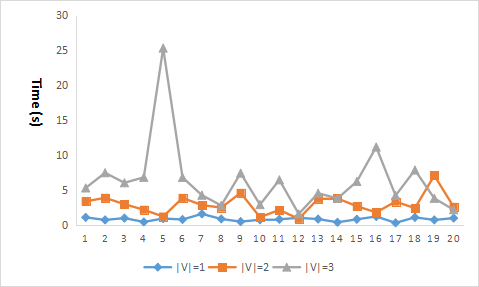
\includegraphics[width=7cm]{chapter04/time_4_12.png}
	}
	\subfigure[$\CTLsnf$子句的个数]{
		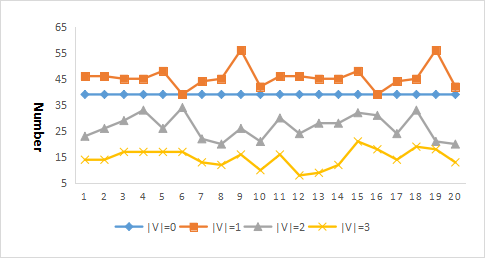
\includegraphics[width=7cm]{chapter04/number-4-12.png}
	}
	\caption{计算{\CTL-forget}$(\varphi, V)$使用的时间和在“移除原子命题”步骤后$\CTLsnf$子句的个数,其中$\varphi_i=12$。}
	\label{chapter04:fig:for12}
\end{figure*}

\begin{figure*}[!htb]
	\centering
	\subfigure[计算遗忘需要的CUP时间]{
		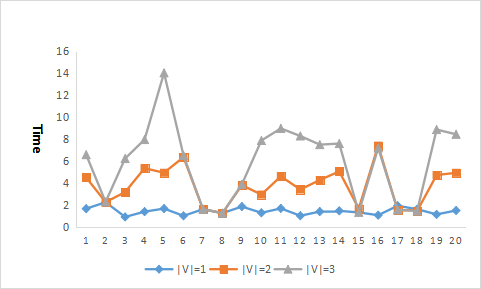
\includegraphics[width=7cm]{chapter04/time_4_16.png}
	}
	\subfigure[$\CTLsnf$子句的个数]{
		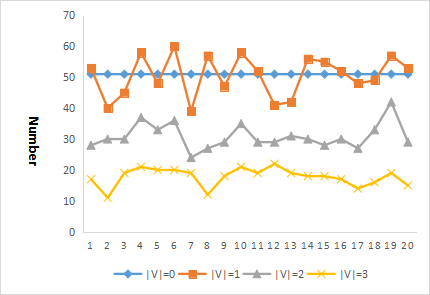
\includegraphics[width=7cm]{chapter04/number-4-16.png}
	}
	\caption{计算{\CTL-forget}$(\varphi, V)$使用的时间和在“移除原子命题”步骤后$\CTLsnf$子句的个数,其中$\varphi_i=16$。}
	\label{chapter04:fig:for16}
\end{figure*}

\subsubsection{SNC计算结果分析}
这部分实验分析使用基于遗忘的方法计算$\CTL$公式的SNC,分为两组实验:计算经典命题公式和$\CTL$公式的SNC,即:计算$q$在$V$和$\varphi \wedge q$上的SNC($\CTLforget(\varphi\wedge q, \Var(\varphi)-V \cup \{q\})$),其中$V\subseteq \Var(\varphi)$、$q\in \Var(\varphi\wedge q)-V$。
这些公式$\varphi$都是随机生成的定义在原子命题集$\Ha$上的公式、$V$也是在计算过程中随机生成的、$q\not \in \Var(\varphi)$是一个固定的原子命题且$|\Ha|=50$。

首先测试随机3-CNF命题公式。令$|V|$的取值范围为$\{5,10,\dots, 40,45\}$,3-CNF公式的子句个数$nc$范围为$\{10,15,\dots, 45,50\}$。
在每种情形当中,计算20个随机实例$(\varphi,q,V)$:$\varphi$为$\Ha$上的公式,且$V\subseteq \Var(\varphi)$。
计算SNC的平均CPU时间如图\ref{chapter04:fig:ProTime}所示。

\begin{figure*}[!htb]
	\centering
	\subfigure[平均CPU时间(s)]{
		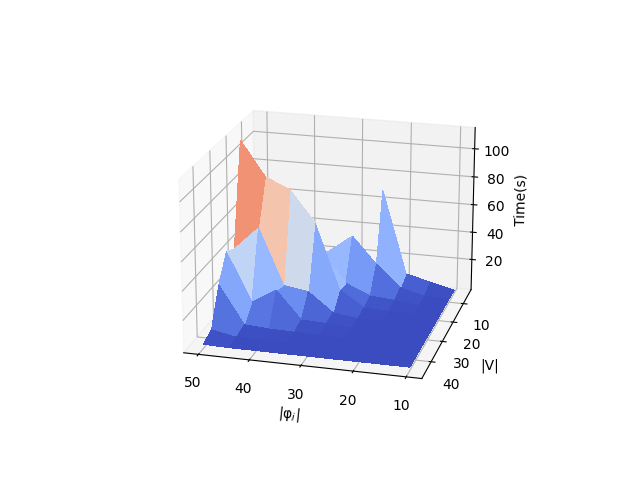
\includegraphics[width=7.5cm]{chapter04/PRototalAveTime.png}
	}
	\subfigure[$|V|=25$时所使用CPU时间箱线图 % and $|\varphi|~\in~ \{10, 15,\dots, 50\}$
	]{
		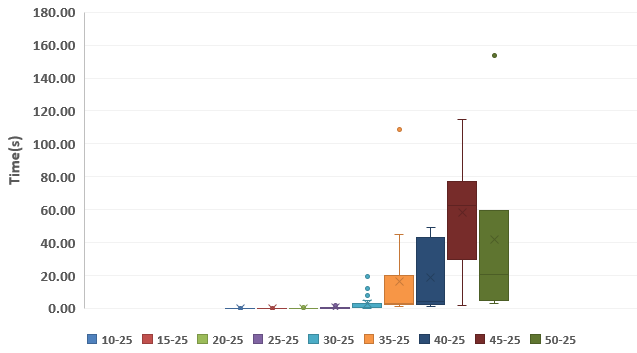
\includegraphics[width=7cm]{chapter04/ProBox(10-50)_25.png}
	}
	\caption{%The performances of computing SNC in PL.
		计算3-CNF公式SNC的CPU时间}
	\label{chapter04:fig:ProTime}
\end{figure*}


从图\ref{chapter04:fig:ProTime}(a)可看出,随着$|\varphi|$增大或$|V|$的减小时间消耗越大。
直观上,若$|\varphi|$越大或者$|V|$越小,则$\CTLforget(\varphi, \overline{V})$越难计算。
这与上一小节中的结论相符合。
图\ref{chapter04:fig:ProTime}(b)展示了当$|V|= 25$、$nc\in \{10,15,\dots, 45, 50\}$时20个随机实例的箱线图。
这同样证明了$nc$越大SNC越难计算。


其次,测试具有如下形式的$\CTL$公式的SNC的计算:
$$\varphi_1 \wedge \ALL \NEXT \varphi_2 \wedge \EXIST\NEXT \varphi_3$$
其中$\varphi_i$($i=1,2,3$)为随机产生的定义在$\Ha$上的3-CNF公式,且满足$|\varphi_1|=|\varphi_2|=|\varphi_3|$。
在这种情形下,每个实例$(\varphi, q, V)$是随机产生的,其中$\varphi=\varphi_1 \wedge \ALL \NEXT \varphi_2 \wedge \EXIST\NEXT \varphi_3$、$V\subseteq \Var(\varphi)$、$|\varphi|\in \{5,6,\dots, 13,14\}$、且$|V|\in \{15,16,\dots, 23,24\}$。
值得注意的是在实例$(\varphi, q, V)$中,$q$可能没有在$V$和$\varphi\wedge q$上的SNC。

图\ref{chapter04:fig:CtlTime}(a)展示了每种情形计算40个实例的SNC的平均CPU时间。与命题公式的情形相似,若$|\varphi|$越大或者$|V|$越小,则$\CTLforget(\varphi, \overline{V})$越难计算。
此外,图\ref{chapter04:fig:CtlTime}(b)展示了每种情形下40个实例中SNC存在的占比,即:$|\varphi|$越小或者$|V|$越小则SNC存在的占比越大。特别地,当$|\varphi_i|=5$且$|V|=16$时,SNC存在的占比为80\%。



\begin{figure*}[!htb]
	\centering
	\subfigure[平均CPU时间(s)]{
		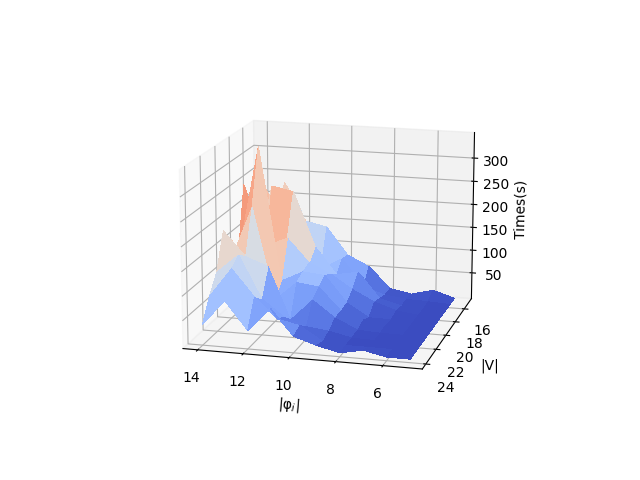
\includegraphics[width=7cm]{chapter04/totalAveTime.png}
	}
	\subfigure[存在SNC的公式占比(\%)]{
		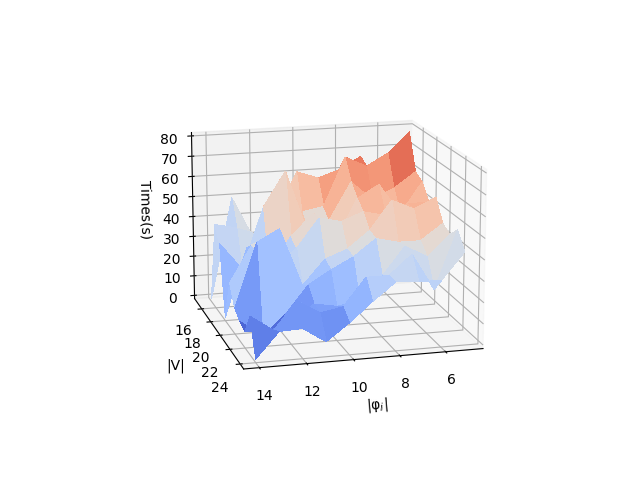
\includegraphics[width=7cm]{chapter04/numPercent.png}
	}
	\caption{计算$\CTL$SNC的平均时间和存在SNC的公式占比.}
	\label{chapter04:fig:CtlTime}
\end{figure*}

综上所述,算法\ref{alg:compute:forgetting:by:Resolution}大多数情况下能计算出SNC(WSC),且当需要遗忘的原子个数很少或公式长度较小的时候计算效率很高。


\section{本章小结} 
本章第~\ref{chapter05:sec:model}讨论了一种基于模型的计算约束$\CTL$下遗忘的计算。为此,本章第一节首先提出了一种有界$V$-互模拟概念,并证明了该有界$V$-互模拟与$V$-互模拟在有限结构下是等价的。此外,定义了给定深度的计算树在给定原子命题集上的特征公式,由此定义了有限结构的特征公式。结论表明初始结构能够满足给定的特征公式当且仅当该初始结构与特征公式对应的初始结构在给定原子命题集上互模拟。基于此,得出了任意公式语义等价于其所有模型的特征公式的析取,因而可以计算遗忘的结果。最后,本章给出了基于模型的计算遗忘算法,并分析该算法关于公式的大小是指数空间的。

本章第~\ref{chapter05:sec:resolution}探索了如何使用Zhang等人提出的归结系统计算$\CTL$下的遗忘。为此,首先使用Zhang提出的转换规则将$\CTL$公式转换成$\CTLsnf$子句集,这一步骤在第\ref{chapter02}章讲述$\CTL$的标准形式时已经给出。基于此,使用归结规则在要遗忘的原子命题集上做穷尽的归结。然后给出几个互模拟等价的等式消除索引,并提出一般化的Ackermann引理用于移除一些新引入的原子命题。最后,给出计算遗忘的算法,并分析该算法的复杂性,分析表明使用该算法计算遗忘的时间和空间复杂性关于公式和要遗忘的原子命题的个数是指数时间的。


随后,第~\ref{cha5:subsec:prolog}节给出了基于Proplog的算法$\CTL$-forget实现介绍。第~\ref{cha5:subsec:expriment}节从两个角度来评估算法$\CTL$-forget的实现系统。实验结果表明,从标准数据集中获取的公式和随机产生的公式下遗忘的计算对需要遗忘的原子命题个数和公式长度都很敏感:要遗忘的原子命题越多或公式越长,计算效率越低。
此外,关于计算SNC的实验表明,本文提出的算法在用于实验的数据集中大部分情况下是能计算出SNC的。三维图和箱线图都表示计算SNC体现了跟计算遗忘一样的规律,这与SNC是由遗忘来计算是一致的。
